\documentclass[12pt, a4paper, oneside]{report}

%=============================================================
% PACKAGES
%=============================================================
\usepackage[top=1.2in, bottom=1.1in, left=1.3in, right=1.1in,
            headheight=15pt]{geometry}
\usepackage{newtxtext, newtxmath}        % Times New Roman
\usepackage[T1]{fontenc}
\usepackage[utf8]{inputenc}
\usepackage{setspace}
\usepackage{parskip}
\usepackage{tocloft}
\usepackage[hidelinks]{hyperref}
\usepackage{graphicx}
\usepackage{fancyhdr}
\usepackage{titlesec}
\usepackage{enumitem}
\usepackage{booktabs}
\usepackage{array}
\usepackage{longtable}
\usepackage{tabularx}
\usepackage{colortbl}
\usepackage{float}
\usepackage{caption}
\usepackage{xcolor}
\usepackage{microtype}
\usepackage{emptypage}
\usepackage{mdframed}
\usepackage{tikz}
\usetikzlibrary{calc, positioning, arrows.meta, shapes.geometric}
\usepackage[pages=all]{background}

% ── Code listings ─────────────────────────────────────────────
\usepackage{listings}
\usepackage{lstautogobble}

% ── Coloured callout boxes ─────────────────────────────────────
\usepackage[most]{tcolorbox}

%=============================================================
% COLOUR PALETTE  (matches the MediLingo AI web application)
%=============================================================
\definecolor{primary}  {RGB}{26,  95, 122}   % deep teal-blue   — headings, borders
\definecolor{accent}   {RGB}{0,  180, 216}   % bright teal      — rules, accents
\definecolor{medgreen} {RGB}{6,  167, 125}   % medical green    — bullets, badges
\definecolor{fillbg}   {RGB}{224, 247, 252}  % teal-50          — light fills
\definecolor{headerbg} {RGB}{200, 238, 248}  % slightly darker  — table headers
\definecolor{bodytext} {RGB}{46,  53,  64}   % near-black       — body text
\definecolor{codebg}   {RGB}{236, 248, 252}  % code block bg
\definecolor{codestr}  {RGB}{6,  167, 125}   % string literals
\definecolor{codecom}  {RGB}{139, 148, 158}  % comments
\definecolor{codekw}   {RGB}{26,  95, 122}   % keywords

%=============================================================
% PAGE BORDER  (drawn on every page behind content)
%=============================================================
\backgroundsetup{
  scale=1, angle=0, opacity=1,
  contents={%
    \begin{tikzpicture}[remember picture, overlay]
      % outer border — thick primary teal-blue
      \draw[primary, line width=2.2pt]
        ([xshift= 8mm, yshift=-8mm] current page.north west)
        rectangle
        ([xshift=-8mm, yshift= 8mm] current page.south east);
      % inner border — thin bright teal
      \draw[accent, line width=0.6pt]
        ([xshift=10.5mm, yshift=-10.5mm] current page.north west)
        rectangle
        ([xshift=-10.5mm, yshift=10.5mm] current page.south east);
    \end{tikzpicture}
  }
}

%=============================================================
% SPACING
%=============================================================
\setstretch{1.5}
\setlength{\parindent}{0pt}
\setlength{\parskip}{7pt plus 1pt}

%=============================================================
% CHAPTER TITLE  — full-width primary strip, double rule
%=============================================================
\titleformat{\chapter}[display]
  {\normalfont\centering}
  {%
    {\setlength{\fboxsep}{0.4cm}%
     \colorbox{primary}{%
       \makebox[\dimexpr\textwidth-2\fboxsep\relax][c]{%
         \color{white}\bfseries\large\scshape
         Chapter\ \thechapter
       }%
     }}%
  }
  {-2pt}
  {\color{primary}\LARGE\bfseries\MakeUppercase}
  [%
    \vspace{6pt}%
    {\color{primary}\titlerule[2.5pt]}%
    \vspace{2pt}%
    {\color{accent}\titlerule[0.7pt]}%
  ]

\titlespacing*{\chapter}{0pt}{40pt}{28pt}

%-------------------------------------------------------------
% SECTION  — vertical bar accent + thin rule
%-------------------------------------------------------------
\titleformat{\section}
  {\normalfont\large\bfseries\color{primary}}
  {{\color{accent}\rule[-3pt]{4pt}{14pt}}\hspace{7pt}\thesection}
  {0.7em}{}
  [\vspace{-5pt}{\color{accent}\titlerule[0.6pt]}\vspace{3pt}]

%-------------------------------------------------------------
% SUBSECTION
%-------------------------------------------------------------
\titleformat{\subsection}
  {\normalfont\normalsize\bfseries\color{primary}}
  {{\color{medgreen}\rule[-2pt]{3pt}{10pt}}\hspace{6pt}\thesubsection}
  {0.7em}{}

%-------------------------------------------------------------
% SUBSUBSECTION
%-------------------------------------------------------------
\titleformat{\subsubsection}
  {\normalfont\normalsize\bfseries\itshape\color{accent}}
  {\thesubsubsection}{1em}{}

%=============================================================
% HEADERS AND FOOTERS
%=============================================================
\pagestyle{fancy}
\fancyhf{}
\renewcommand{\headrulewidth}{2pt}
\renewcommand{\headrule}{%
  {\color{primary}\hrule height\headrulewidth width\headwidth}%
  \vskip-\headrulewidth}

\fancyhead[L]{\small\bfseries\color{primary}\nouppercase{\leftmark}}
\fancyhead[R]{\small\bfseries\color{accent}\thepage}
\fancyfoot{}

\fancypagestyle{plain}{%
  \fancyhf{}
  \renewcommand{\headrulewidth}{0pt}
  \renewcommand{\headrule}{}
  \fancyfoot[C]{%
    {\color{accent}\rule{1.5cm}{0.5pt}}\;%
    {\small\bfseries\color{primary}\thepage}\;%
    {\color{accent}\rule{1.5cm}{0.5pt}}%
  }
}

%=============================================================
% TOC / LOF / LOT
%=============================================================
\renewcommand{\contentsname}{\color{primary}Table of Contents}
\renewcommand{\listfigurename}{\color{primary}List of Figures}
\renewcommand{\listtablename}{\color{primary}List of Tables}
\renewcommand{\cftchapfont}{\bfseries\color{primary}}
\renewcommand{\cftchappagefont}{\bfseries\color{primary}}
\renewcommand{\cftsecfont}{\color{bodytext}}
\renewcommand{\cftsecpagefont}{\color{bodytext}}
\setlength{\cftbeforechapskip}{8pt}
\setlength{\cftbeforesecskip}{2pt}

%=============================================================
% CAPTIONS
%=============================================================
\captionsetup{
  labelfont     = {bf, color=primary},
  font          = {small, color=bodytext},
  labelsep      = colon,
  justification = centering
}

%=============================================================
% BULLET LISTS
%=============================================================
\setlist[itemize,1]{label={\color{primary}$\blacksquare$},
                    leftmargin=2.2em, itemsep=3pt}
\setlist[itemize,2]{label={\color{medgreen}$\bullet$},
                    leftmargin=2.2em, itemsep=1pt}

%=============================================================
% CODE LISTINGS
%=============================================================
\lstdefinestyle{medlingo}{
  backgroundcolor = \color{codebg},
  basicstyle      = \ttfamily\small,
  keywordstyle    = \bfseries\color{codekw},
  stringstyle     = \color{codestr},
  commentstyle    = \itshape\color{codecom},
  numberstyle     = \tiny\color{bodytext!60},
  numbers         = left,
  numbersep       = 8pt,
  stepnumber      = 1,
  frame           = single,
  framesep        = 4pt,
  rulecolor       = \color{accent!50},
  breaklines      = true,
  breakatwhitespace = true,
  autogobble      = true,
  tabsize         = 4,
  showstringspaces= false,
  captionpos      = b,
  xleftmargin     = 10pt,
  xrightmargin    = 4pt,
  aboveskip       = 10pt,
  belowskip       = 6pt,
}
\lstset{style=medlingo}

% Language aliases
\lstdefinelanguage{TypeScript}{
  language     = [LaTeX]TeX,
  morekeywords = {const,let,var,function,return,import,export,from,
                  interface,type,class,extends,implements,async,await,
                  default,true,false,null,undefined,typeof,void,
                  string,number,boolean,any,never,unknown},
  sensitive    = true,
  morecomment  = [l]{//},
  morecomment  = [s]{/*}{*/},
  morestring   = [b]",
  morestring   = [b]',
  morestring   = [b]`,
}

%=============================================================
% TCOLORBOX CALLOUTS
%=============================================================
\tcbuselibrary{skins, breakable}

% \infobox{Title}{Body}
\newcommand{\infobox}[2]{%
  \begin{tcolorbox}[
    enhanced, breakable,
    colback  = fillbg,
    colframe = accent,
    coltitle = white,
    fonttitle= \bfseries\small,
    title    = {#1},
    arc      = 4pt,
    left     = 8pt, right = 8pt,
    top      = 6pt, bottom = 6pt,
    boxrule  = 1.2pt,
  ]
  \small #2
  \end{tcolorbox}%
}

% \notebox{Body}  — borderless note with green accent bar
\newcommand{\notebox}[1]{%
  \begin{tcolorbox}[
    enhanced, breakable,
    colback  = fillbg,
    colframe = medgreen,
    leftrule = 4pt,
    rightrule= 0pt,
    toprule  = 0pt,
    bottomrule= 0pt,
    arc      = 0pt,
    left     = 10pt, right = 8pt,
    top      = 5pt,  bottom = 5pt,
  ]
  \small\color{bodytext} #1
  \end{tcolorbox}%
}

% \warnbox{Body}  — amber-tinted warning
\newcommand{\warnbox}[1]{%
  \begin{tcolorbox}[
    enhanced, breakable,
    colback  = yellow!8!white,
    colframe = orange!70!red,
    leftrule = 4pt,
    rightrule= 0pt,
    toprule  = 0pt,
    bottomrule= 0pt,
    arc      = 0pt,
    left     = 10pt, right = 8pt,
    top      = 5pt,  bottom = 5pt,
  ]
  \small\color{bodytext} #1
  \end{tcolorbox}%
}

%=============================================================
% FIGURE PLACEHOLDER  \figplaceholder[height]{description}
%=============================================================
\newcommand{\figplaceholder}[2][8cm]{%
  \begin{mdframed}[
    linecolor=accent, linewidth=1pt,
    backgroundcolor=fillbg,
    innertopmargin=14pt, innerbottommargin=14pt,
    innerleftmargin=12pt, innerrightmargin=12pt,
    roundcorner=5pt
  ]
  \centering
  {\color{primary}\bfseries\small [Figure Placeholder]}\\[5pt]
  {\color{accent}\itshape\small #2}\\[2pt]
  \rule{0pt}{#1}
  \end{mdframed}%
}

%=============================================================
% TABLE COLUMN HEADER  \theader{text}
%=============================================================
\newcommand{\theader}[1]{%
  \cellcolor{primary}\textbf{\color{white}#1}}

% Alternate row tint for long tables
\newcommand{\rowalt}{\rowcolor{fillbg}}

%=============================================================
% GRAPHICS PATH
%=============================================================
\graphicspath{{figures/}}

%=============================================================
% PDF METADATA  &  HYPERREF COLOURS
%=============================================================
\hypersetup{
  pdftitle   = {MediLingo AI -- FYP Documentation},
  pdfauthor  = {[YOUR FULL NAME]},
  colorlinks = true,
  linkcolor  = primary,
  citecolor  = medgreen,
  urlcolor   = accent,
}

%#############################################################
\begin{document}
\color{bodytext}
%#############################################################

\pagenumbering{roman}

%-------------------------------------------------------------
% TITLE PAGE
%-------------------------------------------------------------
\begin{titlepage}
\centering
\vspace*{0.1cm}

% ── Top decorative strip ──────────────────────────────────
\noindent
\begin{tikzpicture}
  \fill[primary] (0, 0.6cm) rectangle (\linewidth, 1.5cm);
  \fill[accent]  (0, 0)     rectangle (\linewidth, 0.6cm);
\end{tikzpicture}

\vspace{0.9cm}
{\large\color{accent}\scshape Final Year Project Documentation\par}
\vspace{0.35cm}
{\color{accent}\rule{0.55\linewidth}{0.6pt}}\par

\vspace{0.75cm}
{\fontsize{32}{38}\selectfont\bfseries\color{primary} MediLingo AI\par}
\vspace{0.3cm}
{\large\bfseries\color{primary} A Cross-Lingual Medical RAG Chatbot\par}
\vspace{0.15cm}
{\normalsize\itshape\color{bodytext} Supporting English, Urdu and Roman Urdu\par}

\vspace{1.1cm}

% ── Author info box ───────────────────────────────────────
\noindent
\begin{tikzpicture}
  \fill[fillbg] (0,0) rectangle (\linewidth, 3.2cm);
  \draw[accent, line width=0.9pt] (0,0) rectangle (\linewidth, 3.2cm);
  \node[primary, font=\normalsize] at (0.5\linewidth, 2.6cm)
       {Presented By};
  \node[primary, font=\large\bfseries] at (0.5\linewidth, 1.8cm)
       {[YOUR FULL NAME]};
  \node[bodytext, font=\normalsize] at (0.5\linewidth, 1.05cm)
       {Reg.\ No:\ [YOUR REGISTRATION NUMBER]};
\end{tikzpicture}

\vspace{1.0cm}
{\normalsize\color{bodytext} Supervised By\par}
\vspace{0.3cm}
{\large\bfseries\color{primary} [SUPERVISOR NAME]\par}
{\normalsize\color{bodytext} [SUPERVISOR DESIGNATION]\par}

\vfill

% University logo — add figures/uni_logo.png and uncomment:
% \includegraphics[width=2.8cm]{uni_logo}\\[0.4cm]

{\normalsize\color{bodytext} Department of [DEPARTMENT NAME]\par}
{\large\bfseries\color{primary} [UNIVERSITY NAME], [CITY]\par}
{\normalsize\color{bodytext} ([START YEAR]--[END YEAR])\par}

\vspace{0.4cm}

% ── Bottom decorative strip ───────────────────────────────
\noindent
\begin{tikzpicture}
  \fill[accent]  (0, 0.5cm) rectangle (\linewidth, 0.85cm);
  \fill[primary] (0, 0)     rectangle (\linewidth, 0.5cm);
\end{tikzpicture}

\end{titlepage}

%-------------------------------------------------------------
% CERTIFICATE OF APPROVAL
%-------------------------------------------------------------
\clearpage
\thispagestyle{empty}

\noindent
\begin{tikzpicture}
  \fill[primary] (0,0) rectangle (\linewidth, 1.5cm);
  \fill[accent]  (0,-0.3cm) rectangle (\linewidth, 0);
  \node[white, font=\Large\bfseries] at (0.5\linewidth, 0.75cm)
       {CERTIFICATE OF APPROVAL};
\end{tikzpicture}

\vspace{2.5cm}

\noindent
\textbf{\color{primary}Supervisor:}\quad\underline{\hspace{7cm}}\vspace{10pt}

\noindent\textbf{[SUPERVISOR NAME]}\newline
[SUPERVISOR DESIGNATION]\newline
Department of [DEPARTMENT NAME]\newline
[UNIVERSITY NAME], [CITY].

\vspace{2cm}

\noindent
\textbf{\color{primary}Chairperson:}\quad\underline{\hspace{7cm}}\vspace{10pt}

\noindent\textbf{[CHAIRPERSON NAME]}\newline
[CHAIRPERSON DESIGNATION]\newline
Department of [DEPARTMENT NAME]\newline
[UNIVERSITY NAME], [CITY].

\vspace{2cm}
\noindent
\textbf{\color{primary}Date:}\quad\underline{\hspace{5cm}}

%-------------------------------------------------------------
% ACKNOWLEDGEMENT
%-------------------------------------------------------------
\clearpage
\chapter*{Acknowledgement}
\addcontentsline{toc}{chapter}{ACKNOWLEDGEMENT}

[Write your acknowledgement here in your own words.]

\vspace{1.5cm}
\hfill\textbf{\color{primary}[YOUR FULL NAME]}

%-------------------------------------------------------------
% ABSTRACT
%-------------------------------------------------------------
\clearpage
\chapter*{Abstract}
\addcontentsline{toc}{chapter}{ABSTRACT}

Pakistan is home to over 230 million people, the majority of whom communicate in Urdu or
Roman Urdu as their primary language. When seeking medical guidance outside a clinical
setting --- to understand a diagnosis, research a medication or evaluate symptoms --- this
population is largely underserved. The global landscape of AI-powered medical tools is
built almost exclusively around English: queries are expected in English, knowledge bases
are indexed in English and responses are generated in English. A Urdu-speaking user asking
about drug interactions or post-operative care is either met with silence, an inaccurate
machine translation, or a response from a general-purpose model that is not anchored in
verified clinical knowledge and may fabricate medical details.

\textbf{MediLingo AI} is a web-based medical chatbot built on a Retrieval-Augmented
Generation (RAG) architecture that natively handles queries in English, Urdu and Roman
Urdu. The backend is developed in Python using FastAPI and integrates three core
components: a ChromaDB vector store that indexes semantically chunked medical PDF
documents, a \texttt{sentence-transformers} embedding model (\texttt{all-MiniLM-L6-v2})
for dense passage retrieval, and the Groq-hosted LLaMA~3.3-70b large language model for
response generation. The React~19 / TypeScript / Vite frontend provides a persistent,
session-based chat interface with voice input and output via the Web Speech API.

A central design decision is the \textit{language-prefix system}: the user's chosen
language is prepended to every query as a natural-language instruction before the query
reaches the LLM, while the embedding pipeline strips this prefix so that vector search
operates on the semantic content of the medical question rather than the language tag.
Authentication uses a JWT dual-token scheme --- short-lived access tokens held in memory
and long-lived refresh tokens stored in HTTP-only cookies --- with all session history
persisted in MongoDB.

The system demonstrates that a multilingual, domain-grounded medical assistant is
achievable using lightweight open-source models, closing a practical healthcare information
gap for tens of millions of Urdu and Roman Urdu speakers.

%-------------------------------------------------------------
% TABLE OF CONTENTS
%-------------------------------------------------------------
\clearpage
\tableofcontents

%-------------------------------------------------------------
% LIST OF FIGURES
%-------------------------------------------------------------
\clearpage
\listoffigures
\addcontentsline{toc}{chapter}{LIST OF FIGURES}

%-------------------------------------------------------------
% LIST OF TABLES
%-------------------------------------------------------------
\clearpage
\listoftables
\addcontentsline{toc}{chapter}{LIST OF TABLES}

%-------------------------------------------------------------
% MAIN MATTER
%-------------------------------------------------------------
\clearpage
\pagenumbering{arabic}

%=============================================================
% CHAPTER 1 — SOFTWARE PROJECT MANAGEMENT PLAN (SPMP)
%=============================================================

\chapter{Software Project Management Plan (SPMP)}

%-------------------------------------------------------------
\section{Introduction}
%-------------------------------------------------------------

Pakistan is home to over 230 million people, and for most of them Urdu or Roman Urdu is
the language they actually think in. Yet if someone in Lahore or Karachi wants to look up
drug interactions or understand a diagnosis, every halfway-decent AI tool on the internet
responds in one language only: English. Symptom checkers, clinical chatbots, question-answering
systems --- built for English, returning English, assuming English is the default.

That is not a small gap. For a population this size, it is a structural barrier to basic
health information. General-purpose AI assistants like ChatGPT can technically respond in
Urdu, but they pull their medical knowledge straight from training weights --- no verified
source, no updated corpus, no way to trace where a claim came from. In a medical setting,
a confident but wrong answer is not just unhelpful. It is dangerous.

What the problem needs is a system that combines the language flexibility of modern LLMs
with retrieval from a trusted, curated medical knowledge base. Figure~\ref{fig:system_overview}
shows the high-level design of MediLingo AI, which connects a React/Vite frontend to a
FastAPI backend running a full RAG pipeline --- PDF ingestion, semantic indexing, and
multilingual response generation via a hosted large language model.

\begin{figure}[H]
  \centering
  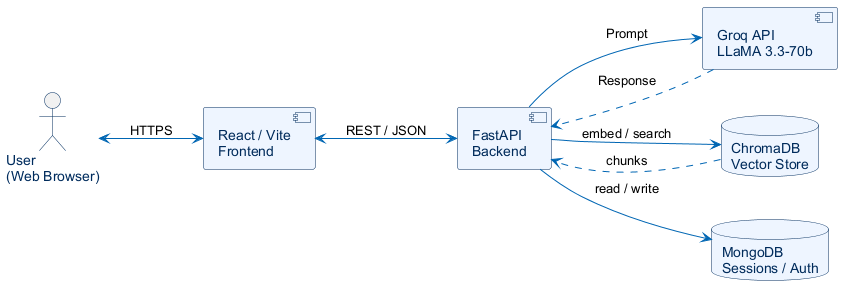
\includegraphics[width=0.90\textwidth]{system_overview}
  \caption{MediLingo AI --- High-Level System Overview}
  \label{fig:system_overview}
\end{figure}

%-------------------------------------------------------------
\subsection{Existing Medical Information Systems}
%-------------------------------------------------------------

\subsubsection{Existing Systems With AI Capabilities}

A number of commercial platforms already use AI for medical information delivery. Each one
has the same blind spot: they are built around English, and there is no real pathway for
someone who wants to type a query in Urdu.

\begin{itemize}

  \item \textbf{Ada Health \cite{adahealth2024}:} Ada is a conversational symptom checker
        that walks users through a structured set of questions and returns a ranked
        differential of probable conditions. Its clinical reasoning engine is proprietary
        and English-only. It does not accept free-text queries in Urdu and provides no
        retrieval mechanism against a user-supplied knowledge base.

        \begin{figure}[H]
          \centering
          \figplaceholder[4cm]{Screenshot of Ada Health symptom checker interface}
          \caption{Ada Health --- AI-driven symptom checker (English only)}
          \label{fig:ada}
        \end{figure}

  \item \textbf{Babylon Health:} Babylon's AI triage service operates on a closed clinical
        model trained on English-language medical data. It has never been deployed in
        Pakistan and does not support Urdu as either an input or output language.

        \begin{figure}[H]
          \centering
          \figplaceholder[4cm]{Screenshot of Babylon Health AI consultation interface}
          \caption{Babylon Health --- AI triage and health consultation}
          \label{fig:babylon}
        \end{figure}

  \item \textbf{Med-PaLM 2 (Google) \cite{singhal2023medpalm}:} Med-PaLM 2 is a large
        language model fine-tuned on medical benchmarks. It scored at expert level on
        medical licensing exams, which is impressive. But it is a research system, not
        publicly available, and it operates in English only --- so for a Urdu-speaking
        user, its benchmark scores are essentially irrelevant.

  \item \textbf{WebMD Symptom Checker:} WebMD uses a keyword-driven symptom tool that
        matches inputs to conditions in a static database. No natural-language generation,
        no retrieval pipeline, no Urdu support. It is more of a lookup tool than an
        intelligent assistant.

\end{itemize}

\subsubsection{Existing Systems Without Multilingual AI}

On the Pakistani side, the platforms that actually serve this population provide health
information without any real AI query capability:

\begin{itemize}

  \item \textbf{Sehat.com.pk and Marham.pk:} These are the most widely used Pakistani
        health portals. They list doctors, allow appointment booking and publish basic
        health articles --- some of it in Urdu. But neither offers an interactive medical
        query interface, and there is no generative response system or retrieval from a
        knowledge base. Useful for finding a doctor; not useful for asking a clinical
        question.

  \item \textbf{General-purpose LLMs (e.g., ChatGPT):} Models like ChatGPT do understand
        Urdu and Roman Urdu reasonably well. The problem is that their medical knowledge
        comes from training data, not a verified clinical corpus. It cannot be updated, and
        there is no way to trace a claim back to a source document. That is a meaningful
        risk in a medical context --- the answer might be fluent and confident while being
        clinically wrong or outdated.

  \item \textbf{Government and hospital websites:} Static health content published by
        Pakistani hospitals and the Ministry of National Health Services is in English.
        None of these platforms offer any interactive query interface at all.

\end{itemize}

%-------------------------------------------------------------
\subsection{Project Overview}
%-------------------------------------------------------------

MediLingo AI is a web-based medical chatbot that takes queries in English, Urdu and Roman
Urdu and returns responses drawn from an indexed collection of medical PDF documents. The
key distinction from a general-purpose chatbot is that responses are not generated from
model memory --- they are grounded in passages retrieved from the vector store at query
time. The LLM is there to synthesise and explain, not to recall.

The backend runs on FastAPI \cite{fastapi2018} and handles four things: user authentication
and session storage via MongoDB \cite{mongodb2024} and JWT tokens; PDF ingestion and
semantic chunking via \texttt{pdfplumber}; dense retrieval via ChromaDB \cite{chromadb2023}
and \texttt{sentence-transformers} \cite{sentencetransformers2019}; and response generation
through the Groq-hosted LLaMA~3.3-70b model \cite{groq2024}. The frontend is React~19 with
TypeScript and Vite \cite{react2024}, styled with TailwindCSS, and uses the browser's Web
Speech API for voice interaction.

The key features of the system are:

\begin{itemize}
  \item User registration, login and password reset via email OTP
  \item Multilingual query input in English, Urdu and Roman Urdu
  \item RAG-grounded responses generated from ingested medical PDFs
  \item Full chat session management: create, continue, rename and delete sessions
  \item Persistent message history stored in MongoDB
  \item Voice input (speech-to-text) and voice output (text-to-speech)
  \item Admin panel for user management and triggering PDF ingestion
  \item JWT dual-token authentication with HTTP-only refresh cookies
\end{itemize}

%-------------------------------------------------------------
\subsection{Project Deliverables}
%-------------------------------------------------------------

\begin{itemize}
  \item Software Project Management Plan (SPMP)
  \item Software Requirements Specification (SRS)
  \item Software Design Description (SDD)
  \item Software Test Documentation (STD)
  \item FastAPI backend with integrated RAG engine and ingestion pipeline
  \item React / TypeScript / Vite frontend with multilingual chat interface
  \item ChromaDB vector store populated from medical PDF documents
  \item MongoDB schema for users, sessions and messages
  \item Docker and Docker Compose configuration for single-command deployment
  \item GitHub repository with complete version-controlled source code
  \item Final working demonstration of the cross-lingual RAG flow
\end{itemize}

%=============================================================
\section{Project Organization}
%=============================================================

%-------------------------------------------------------------
\subsection{Software Process Model}
%-------------------------------------------------------------

The \textbf{Iterative Incremental Model} was chosen for MediLingo AI. The reasoning was
straightforward once the system's structure was clear:

\begin{itemize}

  \item The system breaks down naturally into independent, shippable increments.
        Authentication and session storage can be built and fully verified before a single
        line of RAG code is written. The English-only RAG pipeline can be validated before
        Urdu support is layered on. Voice features can be added last without touching
        anything below them. Each increment leaves the system in a working state.

  \item A RAG pipeline requires empirical tuning --- chunk size, overlap length, top-k
        retrieval count, similarity threshold. These values cannot be derived analytically;
        they have to be evaluated against real queries. An iterative model makes this
        feedback loop part of the process rather than something tacked on at the end.

  \item The language-prefix stripping mechanism was added mid-project, after it became
        clear that embedding the full prefixed query was degrading retrieval quality. An
        iterative approach meant this design change could be isolated to one increment,
        tested and confirmed without breaking anything already shipped.

\end{itemize}

Figure~\ref{fig:process_model} shows the four increments and how each builds on the last.

\begin{figure}[H]
  \centering
  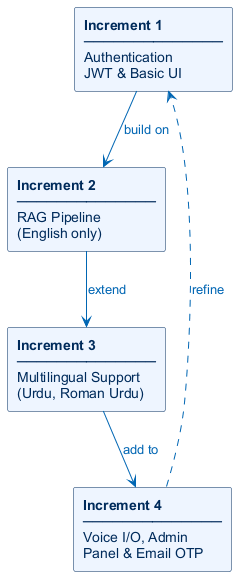
\includegraphics[width=0.75\textwidth]{process_model}
  \caption{Iterative Incremental Software Process Model applied to MediLingo AI}
  \label{fig:process_model}
\end{figure}

%-------------------------------------------------------------
\subsection{Roles and Responsibilities}
%-------------------------------------------------------------

\textbf{Developer (Student):}
\begin{itemize}
  \item Design and implement all FastAPI routers covering authentication
        (\texttt{/auth/*}), session management (\texttt{/sessions/*}) and RAG query
        processing (\texttt{/query}, \texttt{/retrieve}, \texttt{/pipeline/*})
  \item Build the RAG ingestion pipeline: PDF extraction with \texttt{pdfplumber},
        semantic chunking, embedding generation and ChromaDB indexing
  \item Integrate the Groq API and implement the language-prefix stripping mechanism so
        that semantic search operates on clean English text regardless of the query language
  \item Develop the React frontend including the chat page, session sidebar, login,
        register, profile, admin, forgot-password and reset-password pages
  \item Implement voice input and output using the Web Speech API through custom hooks
  \item Set up JWT dual-token authentication with silent refresh on 401 responses
  \item Configure Docker and Docker Compose for the full stack
  \item Write all project documentation and prepare diagrams
\end{itemize}

\textbf{Supervisor:}
\begin{itemize}
  \item Provide architectural guidance on the RAG design and multilingual handling strategy
  \item Review documentation milestones and provide written feedback
  \item Clarify requirements and resolve design ambiguities during development
\end{itemize}

%-------------------------------------------------------------
\subsection{Tools and Techniques}
%-------------------------------------------------------------

\textbf{Tools Used:}

\begin{itemize}
  \item \textbf{Python 3.11 and FastAPI \cite{fastapi2018}} --- asynchronous REST API
        framework with built-in OpenAPI documentation at \texttt{/docs}
  \item \textbf{React 19, TypeScript and Vite \cite{react2024}} --- component-based
        frontend with fast hot-module replacement during development
  \item \textbf{TailwindCSS} --- utility-first CSS framework for all UI styling
  \item \textbf{Zustand} --- minimal state management for auth tokens and session list
  \item \textbf{MongoDB and Motor \cite{mongodb2024}} --- async NoSQL store for
        \texttt{UserDoc}, \texttt{SessionDoc} and \texttt{MessageDoc} records
  \item \textbf{ChromaDB \cite{chromadb2023}} --- embedded vector database; persists to
        \texttt{backend/vectorstore/} and supports cosine similarity search
  \item \textbf{sentence-transformers \texttt{all-MiniLM-L6-v2}
        \cite{sentencetransformers2019}} --- 384-dimensional dense embedding model loaded
        once at startup via the RAG service singleton
  \item \textbf{Groq API (LLaMA~3.3-70b) \cite{groq2024}} --- cloud-hosted inference
        endpoint for final response generation
  \item \textbf{pdfplumber / pypdf} --- PDF text extraction for the ingestion pipeline
  \item \textbf{Docker and Docker Compose} --- containerised deployment of backend,
        frontend and MongoDB as a single \texttt{docker-compose up} command
  \item \textbf{Git and GitHub} --- version control; all increments developed on the same
        main branch with descriptive commits
  \item \textbf{PlantUML} --- UML diagram generation for all SRS and SDD sequence diagrams,
        domain model, class diagram, use case diagram and Gantt chart
  \item \textbf{VS Code + MiKTeX + LaTeX Workshop} --- documentation typesetting for all
        four documents compiled locally with pdflatex
\end{itemize}

\textbf{Techniques Used:}

\begin{itemize}
  \item Retrieval-Augmented Generation (RAG) \cite{lewis2020rag} --- retrieval from a
        curated domain corpus before language model generation
  \item Semantic chunking at 1000 characters with 200-character overlap to preserve
        sentence context across chunk boundaries
  \item Cosine similarity search over 384-dimensional embeddings for passage retrieval
  \item Language-prefix system: user language instruction prepended to query for the LLM
        but stripped before embedding to keep retrieval language-neutral
  \item JWT dual-token authentication: 15-minute access tokens (in-memory only) plus
        7-day refresh tokens (HTTP-only cookie) with automatic silent refresh on 401
  \item RAG singleton lifecycle managed by \texttt{rag\_service.py} with deferred
        import of heavy ML libraries (\texttt{sentence-transformers}, \texttt{chromadb})
        to avoid slowing FastAPI startup
  \item UUID4 string IDs for all MongoDB documents to decouple application identity from
        the MongoDB \texttt{\_id} field
\end{itemize}

%=============================================================
\section{Project Management Plan}
%=============================================================

%-------------------------------------------------------------
\subsection{Tasks}
%-------------------------------------------------------------

The project is organised into six phases executed in iterative sequence:

\begin{itemize}
  \item Requirements Analysis Phase
  \item System Design Phase
  \item Backend Development Phase
  \item Frontend Development Phase
  \item RAG Integration and Multilingual Testing Phase
  \item Testing and Validation Phase
\end{itemize}

%-------------------------------------------------------------
\subsection{Description}
%-------------------------------------------------------------

The \textbf{Requirements Analysis Phase} was really about pinning down what the system
needed to do before any code was written. This meant listing out the functional
requirements --- registration, multilingual medical query, session management, voice I/O,
admin ingestion trigger --- and the non-functional ones around latency, token security and
browser compatibility for voice features.

During the \textbf{System Design Phase}, the three-tier architecture was finalised
alongside the MongoDB document schema, the ChromaDB collection design and the RAG pipeline
dataflow. The language-prefix stripping contract between frontend and backend was one of
the more important design decisions made here. UML artefacts --- use-case diagrams, system
sequence diagrams, domain model and class diagram --- came out of this phase.

The \textbf{Backend Development Phase} is where the actual implementation began. All
FastAPI routers were built, along with \texttt{RAGQueryEngine}, the ingestion pipeline
class \texttt{RAGIngestionPipeline}, the Motor-based database layer and the JWT auth
service. The Groq API integration and the async lifespan startup sequence were also
completed here.

The \textbf{Frontend Development Phase} covered all the React pages and custom hooks:
landing page, chat interface with session sidebar, login and registration flows, profile
page, forgot-password and reset-password pages, admin panel, and the
\texttt{useVoiceInput} / \texttt{useVoiceOutput} hooks. Vite's proxy was configured so
API routes forwarded to \texttt{localhost:8000} during development --- this was important
for getting cookies to work correctly without fighting CORS.

The \textbf{RAG Integration and Multilingual Testing Phase} connected the live frontend
to the backend and ran queries in all three languages. This was the phase where the
language-prefix mechanism was validated --- the test was simple: switching language should
not change which documents get retrieved, only how the response is worded. It passed.

The \textbf{Testing and Validation Phase} covered functional testing of every use case:
JWT token lifecycle, RAG retrieval quality, voice API in Chrome and Edge, and admin
workflows. Issues found here were fixed before final submission.

%-------------------------------------------------------------
\subsection{Project Plan}
%-------------------------------------------------------------

Figure~\ref{fig:gantt} shows the project plan as a Gantt chart. The backend and frontend
development phases overlap intentionally --- waiting for the backend to be completely
finished before touching the frontend would have stretched the timeline by weeks. The
RAG integration phase that follows both is where the two halves are connected and
tested end-to-end.

\begin{figure}[H]
  \centering
  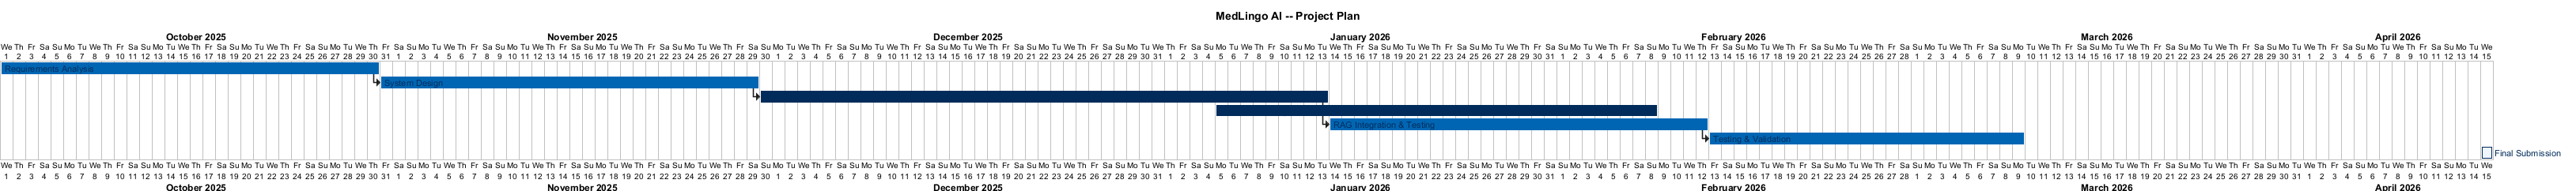
\includegraphics[width=\textwidth]{gantt}
  \caption{Project Management Plan --- Gantt Chart}
  \label{fig:gantt}
\end{figure}

%-------------------------------------------------------------
\subsection{Project Timeline}
%-------------------------------------------------------------

Figure~\ref{fig:timeline} marks the key milestones from requirements analysis to final
submission. The documentation-heavy first half and implementation-heavy second half are
not a coincidence --- writing down what the system needs to do before writing the code
for it saves significant rework later. That principle drove the schedule.

\begin{figure}[H]
  \centering
  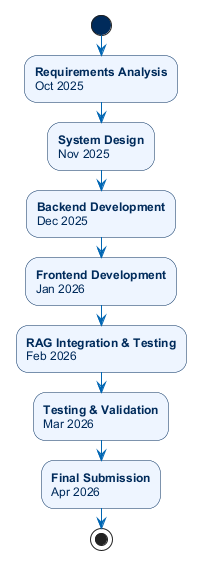
\includegraphics[width=0.45\textwidth]{timeline}
  \caption{MediLingo AI --- Project Timeline}
  \label{fig:timeline}
\end{figure}

%=============================================================
% CHAPTER 2 — SOFTWARE REQUIREMENT SPECIFICATIONS (SRS)
%=============================================================

\chapter{Software Requirement Specifications (SRS)}

Getting requirements right before writing a single line of code is one of those lessons
that takes most developers a bad experience to learn. This chapter documents what
MediLingo AI is actually supposed to do: the problem motivating it, the boundaries it works
within, and the complete set of functional and non-functional requirements. Use cases and
the domain model sit at the end, building on everything before them. The system design
in Chapter~3 should be fully traceable back to this chapter.

%=============================================================
\section{Introduction}
%=============================================================

%-------------------------------------------------------------
\subsection{Problem Statement}
%-------------------------------------------------------------

Pakistan has one of the largest Urdu-speaking populations in the world, yet there is no
publicly accessible, AI-driven medical tool that accepts queries in Urdu or Roman Urdu and
grounds its answers in verified medical documents. The gap has two distinct layers.

The first is language. Every AI medical tool of any quality is built for English. They
cannot process a query written in Urdu, and even when a user translates their question
manually, there is no mechanism to return a response in their native language. The second
layer is reliability. General-purpose LLMs that do support Urdu produce answers from
training weights, not from a curated clinical corpus. In healthcare, a confident but wrong
answer is not just unhelpful --- it carries real risk. Medical facts, dosage details and
symptom descriptions need to come from somewhere traceable, not from statistical patterns
baked into model parameters.

MediLingo AI addresses both. It accepts queries in English, Urdu and Roman Urdu, and every
response is grounded in passages retrieved from an indexed medical knowledge base at query
time --- not recalled from model memory.

%-------------------------------------------------------------
\subsection{Motivation}
%-------------------------------------------------------------

The case for building this came down to three things that kept coming back during the
requirements phase.

\begin{itemize}
  \item \textbf{Language accessibility:} Forcing an Urdu speaker to translate their medical
        question before they can get a useful answer is not a minor inconvenience. For a lot
        of people it is a genuine barrier. Removing the translation step lowers the cost of
        accessing health information for tens of millions of Urdu speakers. That felt like
        a concrete, achievable goal rather than an abstract one.

  \item \textbf{Factual reliability:} The hallucination problem is well-known. RAG is not
        a complete solution, but it meaningfully narrows the gap by tying every response
        to specific retrieved passages from a known knowledge base. At minimum, it makes
        the system's outputs traceable to a source document --- something a standard LLM
        pulling from training memory alone cannot do.

  \item \textbf{Practical feasibility:} The components needed for this --- open-source
        embedding models, a cloud-hosted LLM, a local vector database --- are mature enough
        now that a working system is achievable without proprietary data or specialised
        hardware. That was not obviously true two or three years ago.
\end{itemize}

%-------------------------------------------------------------
\subsection{Objectives}
%-------------------------------------------------------------

The primary objectives of the MediLingo AI project are:

\begin{itemize}
  \item Build a web-based medical chatbot accepting queries in English, Urdu and Roman Urdu,
        returning responses in the same language as the query
  \item Ground every response in verified medical PDF documents through a RAG pipeline ---
        the LLM synthesises and explains, but does not recall clinical facts from memory
  \item Give users a persistent, session-based chat interface so that separate medical
        conversations can be maintained and revisited over time
  \item Implement JWT dual-token authentication with HTTP-only refresh cookies and silent
        renewal so the user's session does not interrupt them
  \item Integrate voice input and output through the Web Speech API, making the system
        accessible to users who prefer speech interaction
  \item Provide an admin interface for user account management and knowledge base
        re-ingestion from PDF files placed in the server datasets directory
\end{itemize}

%-------------------------------------------------------------
\subsection{Scope}
%-------------------------------------------------------------

\textbf{In scope:}
\begin{itemize}
  \item Web application accessible from any modern browser
  \item Query input and response output in English, Urdu and Roman Urdu
  \item RAG pipeline using locally ingested medical PDF documents as the knowledge base
  \item User registration, login, logout and password reset
  \item Chat session creation, continuation, deletion and history viewing
  \item Voice input (speech-to-text) and voice output (text-to-speech)
  \item Admin panel for user management and PDF ingestion trigger
  \item Containerised deployment via Docker and Docker Compose
\end{itemize}

\textbf{Out of scope:}
\begin{itemize}
  \item Native mobile application (iOS or Android)
  \item Diagnostic conclusions or prescriptive medical advice --- the system provides
        information only, not clinical diagnosis
  \item Real-time consultation with a licensed medical professional
  \item Support for languages other than English, Urdu and Roman Urdu
  \item Integration with external electronic health record (EHR) systems
\end{itemize}

%-------------------------------------------------------------
\subsection{Constraints}
%-------------------------------------------------------------

\begin{itemize}
  \item A valid \texttt{GROQ\_API\_KEY} environment variable is required; the backend
        starts successfully without it but every query returns an error until it is set
  \item Voice input and output depend on the Web Speech API, which has full support only
        in Chromium-based browsers (Chrome, Edge) and partial support in Firefox; Safari
        is unsupported for voice input
  \item ChromaDB is used in embedded mode, meaning it is co-located with the backend
        process and does not support distributed or replicated vector storage out of the box
  \item The \texttt{sentence-transformers} model (\texttt{all-MiniLM-L6-v2}) is loaded
        fully into RAM on startup; the server requires a minimum of 512 MB of available
        memory for the ML components alone
  \item Medical knowledge is limited to the content of PDF files placed in
        \texttt{backend/datasets/} and ingested through the admin pipeline; the system
        cannot answer questions on topics not covered by those documents
  \item The language-prefix mechanism relies on the Groq-hosted LLaMA 3.3-70b model's
        built-in multilingual capability; the quality of Urdu and Roman Urdu responses
        depends on the model's training data and may vary by medical sub-domain
\end{itemize}

%-------------------------------------------------------------
\subsection{Assumptions}
%-------------------------------------------------------------

\begin{itemize}
  \item All medical PDF documents provided for ingestion are written in English; the
        embedding model operates on English text, and translating source documents is
        outside the scope of the system
  \item Users have a stable internet connection sufficient for REST API calls and Groq
        inference requests
  \item The Groq API service remains available during system operation; no fallback LLM
        is configured
  \item Users interact with the system through a web browser on a desktop or laptop
        device; mobile browser support is functional but not the primary design target
  \item The admin user is technically familiar enough to place PDF files in the correct
        server directory and invoke the ingestion endpoint
\end{itemize}

%-------------------------------------------------------------
\subsection{System Workflow Diagram}
%-------------------------------------------------------------

Figure~\ref{fig:workflow} shows what actually happens to a query from the moment the user
hits submit to the moment the response lands on screen. The language prefix gets stripped
early in the process so that vector search always runs against clean medical text ---
this is the key design detail that makes multilingual retrieval work correctly.

\begin{figure}[H]
  \centering
  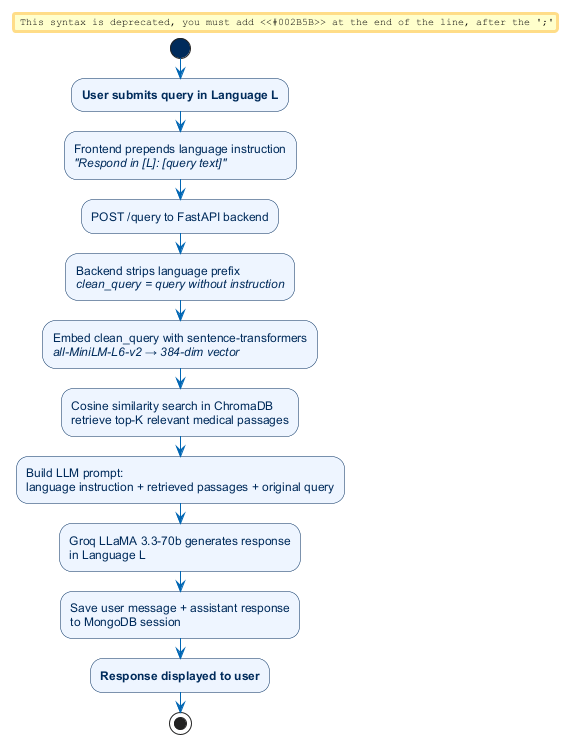
\includegraphics[width=0.55\textwidth]{workflow}
  \caption{MediLingo AI --- End-to-End System Workflow for Multilingual Medical Query}
  \label{fig:workflow}
\end{figure}

%=============================================================
\section{Overall Description}
%=============================================================

%-------------------------------------------------------------
\subsection{Product Perspective}
%-------------------------------------------------------------

MediLingo AI is a self-contained web application. It does not plug into any larger platform
and depends on only three external services: the Groq API for LLM inference, MongoDB for
persistent storage, and ChromaDB for document retrieval. All three can run on the same host
as the FastAPI backend or on separate infrastructure without any changes to the application
code. During development, a Vite proxy forwards all API traffic from the browser to
\texttt{localhost:8000}, which means browser cookies work without fighting CORS --- one
fewer thing to debug during development.

%-------------------------------------------------------------
\subsection{User Characteristics}
%-------------------------------------------------------------

\textbf{Regular User:}
Someone looking for medical information --- could be fluent in English, Urdu or Roman Urdu,
or switching between all three. The interface requires basic internet literacy and nothing
more. Users should not need to understand anything about RAG or how the backend works. Voice
support is there specifically for people who have difficulty typing or just prefer speaking.

\textbf{Admin User:}
Someone with enough technical familiarity to place PDF files in the correct server directory
and trigger the ingestion endpoint from the admin panel. They authenticate through a
dedicated admin login route that verifies the role field in the JWT payload before granting
access to admin-only endpoints.

%=============================================================
\section{Specific Requirements}
%=============================================================

%-------------------------------------------------------------
\subsection{External Interface Requirements}
%-------------------------------------------------------------

\textbf{User Interface:}
A React SPA delivered in the browser. The interface includes a landing page, auth pages
(login, register, forgot password, reset password), a chat page with a collapsible session
sidebar, a profile page and an admin panel. No plugin or browser extension is required.

\textbf{Hardware Interface:}
A standard desktop or laptop with a microphone for voice input, and speakers or
headphones for voice output. No specialised hardware needed.

\textbf{Software Interface:}
The backend exposes a documented REST API at \texttt{/docs} (Swagger UI). The frontend
uses this interface exclusively. The backend communicates with MongoDB via Motor and with
ChromaDB via its Python client.

\textbf{Communication Interface:}
All frontend-to-backend communication is HTTP/HTTPS with JSON bodies. Auth credentials go
as a Bearer token in the \texttt{Authorization} header. Refresh tokens are transmitted as
HTTP-only cookies.

%-------------------------------------------------------------
\subsection{Functional Requirements}
%-------------------------------------------------------------

\renewcommand{\arraystretch}{1.35}
\begin{longtable}{|>{\bfseries\color{navyblue}\centering}p{1.3cm}|p{4.2cm}|p{7.8cm}|}
\caption{Functional Requirements of MediLingo AI}
\label{tab:fr} \\
\hline
\theader{ID} & \theader{Requirement} & \theader{Description} \\
\hline
\endfirsthead
\hline
\theader{ID} & \theader{Requirement} & \theader{Description} \\
\hline
\endhead
\hline
\endfoot

FR-01 & User Registration &
  The system shall allow a new user to create an account using a display name, email
  address and password. Duplicate email addresses must be rejected. \\
\hline
FR-02 & User Login &
  The system shall authenticate a registered user with their email and password, issue a
  JWT access token and set an HTTP-only JWT refresh cookie. \\
\hline
FR-03 & Silent Token Refresh &
  The frontend shall automatically call \texttt{POST /auth/refresh} when the backend
  returns HTTP 401, retry the original request with the new access token, and redirect to
  login only if the refresh token has also expired. \\
\hline
FR-04 & User Logout &
  The system shall invalidate the refresh cookie and clear in-memory auth state on
  explicit logout. \\
\hline
FR-05 & Password Reset via Email OTP &
  The system shall allow a registered user to reset their password by requesting a
  one-time passcode sent to their registered email address. \\
\hline
FR-06 & Multilingual Query Submission &
  The system shall accept medical queries in English, Urdu and Roman Urdu and return
  a response in the same language as the query. \\
\hline
FR-07 & RAG-Grounded Response Generation &
  Every query response shall be generated by first retrieving the top-K semantically
  relevant passages from the ChromaDB vector store and including them in the LLM prompt. \\
\hline
FR-08 & Language-Prefix Stripping &
  The backend shall strip the language instruction prefix from the query text before
  computing the embedding, so that vector search operates on the medical content
  alone. \\
\hline
FR-09 & Chat Session Creation &
  An authenticated user shall be able to start a new chat session. The session shall be
  saved to MongoDB and appear in the session sidebar. \\
\hline
FR-10 & Chat Session Management &
  An authenticated user shall be able to view, continue and delete any of their saved
  chat sessions. All messages within a deleted session shall be removed. \\
\hline
FR-11 & Message Persistence &
  Every user query and assistant response within a session shall be saved as a
  \texttt{MessageDoc} in MongoDB so that session history survives page reload. \\
\hline
FR-12 & Voice Input &
  The system shall provide a microphone button that activates the browser's Web Speech
  API to transcribe speech into the query input field. \\
\hline
FR-13 & Voice Output &
  The system shall read assistant responses aloud using the browser's SpeechSynthesis API
  after each response is received. \\
\hline
FR-14 & User Profile Management &
  An authenticated user shall be able to view and update their display name and email
  address from the profile page. \\
\hline
FR-15 & Admin: User Management &
  An admin user shall be able to view all registered accounts and activate or deactivate
  individual users. \\
\hline
FR-16 & Admin: PDF Ingestion &
  An admin user shall be able to trigger a synchronous or background ingestion of PDF
  files from \texttt{backend/datasets/} into the ChromaDB vector store via the admin
  panel. \\
\hline
\end{longtable}

%-------------------------------------------------------------
\subsection{Non-Functional Requirements}
%-------------------------------------------------------------

\renewcommand{\arraystretch}{1.35}
\begin{longtable}{|>{\bfseries\color{navyblue}\centering}p{1.3cm}|p{3.5cm}|p{8.5cm}|}
\caption{Non-Functional Requirements of MediLingo AI}
\label{tab:nfr} \\
\hline
\theader{ID} & \theader{Category} & \theader{Requirement} \\
\hline
\endfirsthead
\hline
\theader{ID} & \theader{Category} & \theader{Requirement} \\
\hline
\endhead
\hline
\endfoot

NFR-01 & Performance &
  End-to-end query response time (from submission to display) shall not exceed 15 seconds
  under normal Groq API latency conditions. \\
\hline
NFR-02 & Security &
  User passwords shall be stored as bcrypt hashes. Access tokens shall never be persisted
  to localStorage or sessionStorage. Refresh tokens shall be stored in HTTP-only, Secure
  cookies only. \\
\hline
NFR-03 & Reliability &
  The RAG engine and ingestion pipeline shall be initialised as a singleton at backend
  startup. If initialisation fails, the backend shall still start and return a descriptive
  error on query endpoints rather than crashing entirely. \\
\hline
NFR-04 & Availability &
  The system shall be deployable as a set of Docker containers that can be started with a
  single \texttt{docker-compose up} command, minimising manual deployment steps. \\
\hline
NFR-05 & Maintainability &
  Backend logic shall be separated into distinct FastAPI routers
  (\texttt{auth}, \texttt{sessions}, \texttt{query}). Frontend business logic shall be
  isolated in custom React hooks, separate from UI components. \\
\hline
NFR-06 & Portability &
  The application shall run on any machine with Docker installed, regardless of the
  underlying operating system. \\
\hline
NFR-07 & Browser Compatibility &
  The web application shall function correctly on Chrome 120+, Edge 120+ and Firefox 121+.
  Voice features shall degrade gracefully (button hidden or disabled) on unsupported
  browsers. \\
\hline
NFR-08 & Usability &
  The language selector, voice button and session sidebar shall be visible and operable
  without reading any documentation. The interface shall be fully functional on a
  1280$\times$720 desktop viewport. \\
\hline
\end{longtable}

%=============================================================
\section{Software Product Features}
%=============================================================

MediLingo AI exposes the following top-level product features:

\begin{itemize}
  \item \textbf{Cross-Lingual Medical Chat} --- queries and responses in English, Urdu or
        Roman Urdu, with language routing handled automatically by the prefix mechanism in
        the frontend and backend

  \item \textbf{RAG-Grounded Answers} --- each response is generated from retrieved passages
        rather than from the LLM's memory; medical content is always traceable to a source
        document

  \item \textbf{Persistent Session History} --- users maintain multiple named conversations
        and can return to any of them at any time; message history survives page reloads
        because it is stored in MongoDB, not in browser memory

  \item \textbf{Voice Interaction} --- speech-to-text for query input and text-to-speech
        for response playback; both use the browser's built-in Web Speech API with no
        additional plugin required

  \item \textbf{Secure Authentication} --- 15-minute access tokens kept in memory,
        7-day refresh tokens in HTTP-only cookies, automatic silent renewal so the user's
        session does not get interrupted

  \item \textbf{Admin Knowledge Management} --- administrators can expand or refresh the
        medical knowledge base by triggering a new PDF ingestion run through the admin panel

  \item \textbf{Email-Based Password Recovery} --- users can regain access via a time-limited
        one-time passcode sent to their registered email address
\end{itemize}

%=============================================================
\section{Software System Attributes}
%=============================================================

%-------------------------------------------------------------
\subsection{Reliability}
%-------------------------------------------------------------

The RAG engine and ingestion pipeline are initialised as module-level singletons in
\texttt{rag\_service.py}, loaded once when the FastAPI server starts. If the Groq API
is temporarily unavailable, the backend logs the error and returns a structured HTTP 500
rather than taking down the server process. MongoDB is handled the same way. The guiding
principle was straightforward: one broken external dependency should not kill the whole
application, and a structured error message is almost always more useful than a crash.

%-------------------------------------------------------------
\subsection{Availability}
%-------------------------------------------------------------

The system is packaged with Docker Compose. A single \texttt{docker-compose up} command
starts the FastAPI backend, the React frontend and MongoDB together. Once running, the
application is available at \texttt{localhost:5173} (frontend) and \texttt{localhost:8000}
(API). No further configuration is required beyond setting the environment variables
described in the CLAUDE.md file.

%-------------------------------------------------------------
\subsection{Security}
%-------------------------------------------------------------

Passwords go through bcrypt before they ever touch the database --- there is no plaintext
stored anywhere in the system. Access tokens live exclusively in Zustand in-memory state
and disappear when the browser tab closes. Refresh tokens go into HTTP-only cookies that
JavaScript cannot read, which closes off the most common XSS token-theft vector. CORS is
configured in \texttt{main.py} to restrict cross-origin requests to the deployed frontend
origin; wildcard origins are not used.

%-------------------------------------------------------------
\subsection{Maintainability}
%-------------------------------------------------------------

The backend splits cleanly into independent FastAPI routers, one file each for auth,
sessions and query/pipeline. Adding a new API surface means writing one router file and
one \texttt{app.include\_router()} call --- nothing else changes. On the frontend, all
data-fetching and auth logic lives in custom hooks (\texttt{useAuth}, \texttt{useChat},
\texttt{useSessions}), keeping UI components stateless. That separation makes it
much easier to test business logic independently of the rendering layer.

%-------------------------------------------------------------
\subsection{Portability}
%-------------------------------------------------------------

Everything runs inside Docker containers. The host machine needs Docker Engine and nothing
else. Python 3.11 and Node 20 are fixed in the build image specifications so that a build
on one machine produces the same result as a build on any other --- the
``works on my machine'' problem is eliminated by design.

%-------------------------------------------------------------
\subsection{Performance}
%-------------------------------------------------------------

Heavy ML imports --- \texttt{sentence-transformers} and \texttt{chromadb} --- are deferred
inside \texttt{init\_rag()} and loaded once at startup rather than at module import time.
This keeps FastAPI's startup fast and avoids reloading the embedding model on every
request. The \texttt{all-MiniLM-L6-v2} model produces 384-dimensional embeddings; at that
dimensionality, a ChromaDB cosine search across several thousand chunks runs in well under
100\,ms on a standard CPU. That leaves the Groq API call as the primary latency variable,
not the retrieval step.

%=============================================================
\section{Database Requirements}
%=============================================================

MediLingo AI uses two persistence layers.

\textbf{MongoDB} stores three collections:
\begin{itemize}
  \item \texttt{users} --- one document per registered account, containing the UUID4
        string ID, display name, email, bcrypt password hash, role and active flag
  \item \texttt{sessions} --- one document per chat session, containing the session ID,
        the owning user's ID and a display title
  \item \texttt{messages} --- one document per message (user query or assistant response),
        containing the parent session ID, the message role
        (\texttt{user} or \texttt{assistant}), the content text, the language code and a
        timestamp
\end{itemize}

\textbf{ChromaDB} stores one collection (\texttt{medical\_documents}):
\begin{itemize}
  \item Each record holds the chunk text, its 384-dimensional embedding vector, and
        metadata including the source filename and chunk index
  \item The collection is populated by the ingestion pipeline and queried at inference
        time using cosine similarity
  \item The collection persists to \texttt{backend/vectorstore/} on the host filesystem
\end{itemize}

%=============================================================
\section{Use Cases}
%=============================================================

%-------------------------------------------------------------
\subsection{Use Cases List}
%-------------------------------------------------------------

\renewcommand{\arraystretch}{1.3}
\begin{table}[H]
\centering
\small
\caption{User Use Cases}
\label{tab:user_uc}
\begin{tabular}{|>{\bfseries\color{navyblue}\centering}p{1.5cm}|p{4.5cm}|p{7cm}|}
\hline
\theader{UC ID} & \theader{Use Case Name} & \theader{Brief Description} \\
\hline
UC-1 & Register User Account    & Create a new MediLingo AI account with name, email and password. \\ \hline
UC-2 & Login                    & Authenticate an existing account and receive JWT tokens. \\ \hline
UC-3 & Submit Medical Query     & Send a multilingual medical question and receive a RAG-grounded response. \\ \hline
UC-4 & Manage Chat Sessions     & Create, continue, view and delete persistent chat sessions. \\ \hline
UC-5 & Use Voice Input          & Dictate a query via microphone using the Web Speech API. \\ \hline
UC-6 & Use Voice Output         & Have an assistant response read aloud via text-to-speech. \\ \hline
UC-7 & Manage Profile           & View and update display name and email address. \\ \hline
UC-8 & Reset Password           & Recover account access via an email one-time passcode. \\ \hline
\end{tabular}
\end{table}

\begin{table}[H]
\centering
\small
\caption{Admin Use Cases}
\label{tab:admin_uc}
\begin{tabular}{|>{\bfseries\color{navyblue}\centering}p{1.5cm}|p{4.5cm}|p{7cm}|}
\hline
\theader{UC ID} & \theader{Use Case Name} & \theader{Brief Description} \\
\hline
UC-9  & Manage Users            & View all accounts; activate or deactivate individual users. \\ \hline
UC-10 & Ingest Medical Documents & Trigger PDF extraction, chunking, embedding and ChromaDB indexing. \\ \hline
\end{tabular}
\end{table}

%-------------------------------------------------------------
\subsection{Use Case Diagram}
%-------------------------------------------------------------

\begin{figure}[H]
  \centering
  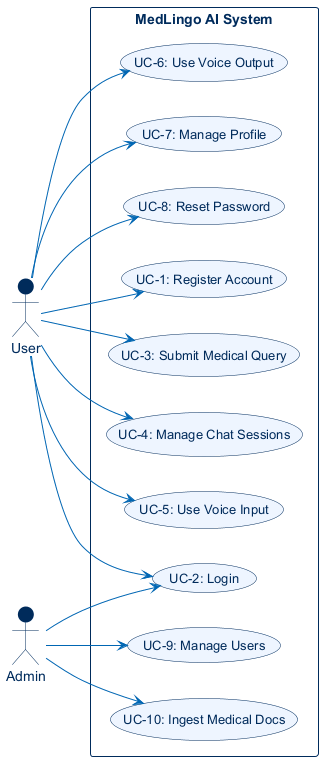
\includegraphics[width=0.85 \textwidth]{use_case_diagram}
  \caption{MediLingo AI --- Use Case Diagram}
  \label{fig:ucd}
\end{figure}

%-------------------------------------------------------------
\subsection{Use Cases Description}
%-------------------------------------------------------------

\renewcommand{\arraystretch}{1.4}

% ─── UC-1 ───────────────────────────────────────────────────
\begin{table}[H]
\centering\small
\caption{UC-1: Register User Account}
\label{tab:uc1}
\begin{tabular}{|>{\bfseries\color{navyblue}}p{3.2cm}|p{9.8cm}|}
\hline
\multicolumn{2}{|c|}{\cellcolor{navyblue}\textbf{\color{white}UC-1: Register User Account}} \\ \hline
Use Case ID     & UC-1 \\ \hline
Actor           & Unregistered User \\ \hline
Description     & A new user creates a MediLingo AI account by supplying a display name, email address and password. \\ \hline
Preconditions   & The provided email address is not already associated with an existing account. \\ \hline
Main Flow       &
  1.\ User navigates to the Register page. \newline
  2.\ User enters display name, email address and password. \newline
  3.\ System validates that the email is not already in use. \newline
  4.\ System hashes the password with bcrypt and creates a UserDoc in MongoDB. \newline
  5.\ System issues a 15-minute access token and sets a 7-day HTTP-only refresh cookie. \newline
  6.\ User is redirected to the chat interface. \\ \hline
Alternate Flow  &
  \textbf{A1} -- Email already registered: system returns HTTP~400 and the user corrects the email field. \newline
  \textbf{A2} -- Password below minimum length: the form is rejected client-side before submission. \\ \hline
Postconditions  & A UserDoc exists in the \texttt{users} collection. The user is authenticated with valid JWT tokens. \\ \hline
\end{tabular}
\end{table}

% ─── UC-2 ───────────────────────────────────────────────────
\begin{table}[H]
\centering\small
\caption{UC-2: Login}
\label{tab:uc2}
\begin{tabular}{|>{\bfseries\color{navyblue}}p{3.2cm}|p{9.8cm}|}
\hline
\multicolumn{2}{|c|}{\cellcolor{navyblue}\textbf{\color{white}UC-2: Login}} \\ \hline
Use Case ID     & UC-2 \\ \hline
Actor           & Registered User / Admin User \\ \hline
Description     & An existing user authenticates with their email and password to receive JWT tokens. \\ \hline
Preconditions   & A valid account exists for the provided email. The account is active. \\ \hline
Main Flow       &
  1.\ User navigates to the Login page. \newline
  2.\ User enters email address and password. \newline
  3.\ System verifies the bcrypt hash against the stored value. \newline
  4.\ System issues a new access token and sets a new refresh cookie. \newline
  5.\ User is redirected to the chat interface. \\ \hline
Alternate Flow  &
  \textbf{A1} -- Incorrect credentials: system returns HTTP~401 and the user is prompted to retry. \newline
  \textbf{A2} -- Account deactivated: system returns HTTP~403 with an appropriate error message. \\ \hline
Postconditions  & The user's access token is held in Zustand memory. A refresh cookie is set in the browser. \\ \hline
\end{tabular}
\end{table}

% ─── UC-3 ───────────────────────────────────────────────────
\begin{table}[H]
\centering\small
\caption{UC-3: Submit Medical Query}
\label{tab:uc3}
\begin{tabular}{|>{\bfseries\color{navyblue}}p{3.2cm}|p{9.8cm}|}
\hline
\multicolumn{2}{|c|}{\cellcolor{navyblue}\textbf{\color{white}UC-3: Submit Medical Query}} \\ \hline
Use Case ID     & UC-3 \\ \hline
Actor           & Authenticated User \\ \hline
Description     & The user submits a medical question in their chosen language and receives a RAG-grounded response in the same language. \\ \hline
Preconditions   & User is authenticated. The RAG engine is initialised. At least one document has been ingested into ChromaDB. \\ \hline
Main Flow       &
  1.\ User selects a language (English / Urdu / Roman Urdu) and types a query. \newline
  2.\ Frontend prepends the language instruction to the query text. \newline
  3.\ Frontend sends POST \texttt{/query} with the prefixed query and session ID. \newline
  4.\ Backend strips the language prefix; the clean query is embedded with \texttt{all-MiniLM-L6-v2}. \newline
  5.\ Backend performs cosine similarity search in ChromaDB and retrieves the top-K passages. \newline
  6.\ Backend builds a prompt containing the language instruction, retrieved passages and query. \newline
  7.\ Groq LLaMA~3.3-70b generates a response in the selected language. \newline
  8.\ Backend saves user message and assistant response as MessageDocs in MongoDB. \newline
  9.\ Response is returned to the frontend and displayed in the chat interface. \\ \hline
Alternate Flow  &
  \textbf{A1} -- Groq API unavailable: system returns HTTP~500 with ``Service temporarily unavailable''. \newline
  \textbf{A2} -- No relevant passages found: LLM is prompted to indicate insufficient information in the knowledge base. \newline
  \textbf{A3} -- Access token expired: \texttt{authenticatedFetch} silently calls \texttt{/auth/refresh} and retries. \\ \hline
Postconditions  & The query and response are saved to the session. The chat view is updated. \\ \hline
\end{tabular}
\end{table}

% ─── UC-4 ───────────────────────────────────────────────────
\begin{table}[H]
\centering\small
\caption{UC-4: Manage Chat Sessions}
\label{tab:uc4}
\begin{tabular}{|>{\bfseries\color{navyblue}}p{3.2cm}|p{9.8cm}|}
\hline
\multicolumn{2}{|c|}{\cellcolor{navyblue}\textbf{\color{white}UC-4: Manage Chat Sessions}} \\ \hline
Use Case ID     & UC-4 \\ \hline
Actor           & Authenticated User \\ \hline
Description     & The user creates, switches between and deletes named chat sessions via the session sidebar. \\ \hline
Preconditions   & User is authenticated. \\ \hline
Main Flow       &
  1.\ User clicks ``New Session'' in the sidebar; a new SessionDoc is created in MongoDB. \newline
  2.\ User clicks an existing session to load its message history. \newline
  3.\ User deletes a session; the SessionDoc and all child MessageDocs are removed. \\ \hline
Alternate Flow  &
  \textbf{A1} -- Network error during session creation: the sidebar shows an error and the session is not added. \\ \hline
Postconditions  & The selected session is active and its messages are loaded in the chat area. \\ \hline
\end{tabular}
\end{table}

% ─── UC-5 ───────────────────────────────────────────────────
\begin{table}[H]
\centering\small
\caption{UC-5: Use Voice Input}
\label{tab:uc5}
\begin{tabular}{|>{\bfseries\color{navyblue}}p{3.2cm}|p{9.8cm}|}
\hline
\multicolumn{2}{|c|}{\cellcolor{navyblue}\textbf{\color{white}UC-5: Use Voice Input}} \\ \hline
Use Case ID     & UC-5 \\ \hline
Actor           & Authenticated User \\ \hline
Description     & The user dictates their query via the microphone button; the transcript populates the query input field. \\ \hline
Preconditions   & User is authenticated. Browser supports the Web Speech API. Microphone permission has been granted. \\ \hline
Main Flow       &
  1.\ User clicks the microphone button in the chat interface. \newline
  2.\ Browser requests microphone permission if not already granted. \newline
  3.\ Speech recognition starts; the user speaks their query. \newline
  4.\ Transcript text is placed in the query input field. \newline
  5.\ User submits the query normally (UC-3). \\ \hline
Alternate Flow  &
  \textbf{A1} -- Microphone permission denied: an error alert is shown and recognition does not start. \newline
  \textbf{A2} -- Browser does not support Web Speech API: the microphone button is hidden. \\ \hline
Postconditions  & Query input field contains the transcribed text, ready for submission. \\ \hline
\end{tabular}
\end{table}

% ─── UC-6 ───────────────────────────────────────────────────
\begin{table}[H]
\centering\small
\caption{UC-6: Use Voice Output}
\label{tab:uc6}
\begin{tabular}{|>{\bfseries\color{navyblue}}p{3.2cm}|p{9.8cm}|}
\hline
\multicolumn{2}{|c|}{\cellcolor{navyblue}\textbf{\color{white}UC-6: Use Voice Output}} \\ \hline
Use Case ID     & UC-6 \\ \hline
Actor           & Authenticated User \\ \hline
Description     & After an assistant response is displayed, the system reads it aloud in the user's selected language using the browser's SpeechSynthesis API. \\ \hline
Preconditions   & A response has been received and rendered. Browser supports SpeechSynthesis. \\ \hline
Main Flow       &
  1.\ Assistant response is received by the frontend. \newline
  2.\ \texttt{useVoiceOutput} hook passes the response text to the SpeechSynthesis API. \newline
  3.\ Browser reads the text aloud in the configured language voice. \\ \hline
Alternate Flow  &
  \textbf{A1} -- SpeechSynthesis not available: response is displayed as text only; no error is shown. \\ \hline
Postconditions  & The response text has been read aloud or silently displayed if TTS is unavailable. \\ \hline
\end{tabular}
\end{table}

% ─── UC-7 ───────────────────────────────────────────────────
\begin{table}[H]
\centering\small
\caption{UC-7: Manage Profile}
\label{tab:uc7}
\begin{tabular}{|>{\bfseries\color{navyblue}}p{3.2cm}|p{9.8cm}|}
\hline
\multicolumn{2}{|c|}{\cellcolor{navyblue}\textbf{\color{white}UC-7: Manage Profile}} \\ \hline
Use Case ID     & UC-7 \\ \hline
Actor           & Authenticated User \\ \hline
Description     & The user views and updates their display name or email address from the profile page. \\ \hline
Preconditions   & User is authenticated. \\ \hline
Main Flow       &
  1.\ User navigates to the Profile page. \newline
  2.\ Current display name and email are pre-filled in the form. \newline
  3.\ User edits one or both fields and clicks Save. \newline
  4.\ System updates the UserDoc in MongoDB and returns the updated values. \\ \hline
Alternate Flow  &
  \textbf{A1} -- New email already taken: system returns HTTP~400 and the user corrects input. \\ \hline
Postconditions  & The UserDoc in MongoDB reflects the updated display name or email. \\ \hline
\end{tabular}
\end{table}

% ─── UC-8 ───────────────────────────────────────────────────
\begin{table}[H]
\centering\small
\caption{UC-8: Reset Password}
\label{tab:uc8}
\begin{tabular}{|>{\bfseries\color{navyblue}}p{3.2cm}|p{9.8cm}|}
\hline
\multicolumn{2}{|c|}{\cellcolor{navyblue}\textbf{\color{white}UC-8: Reset Password}} \\ \hline
Use Case ID     & UC-8 \\ \hline
Actor           & Registered User \\ \hline
Description     & A user who has forgotten their password recovers account access via a one-time passcode sent to their registered email address. \\ \hline
Preconditions   & An account exists for the email address provided. \\ \hline
Main Flow       &
  1.\ User navigates to Forgot Password and enters their registered email. \newline
  2.\ System generates a time-limited OTP and sends it via the email service. \newline
  3.\ User enters the OTP on the Reset Password page. \newline
  4.\ User sets and confirms a new password. \newline
  5.\ System hashes the new password and updates the UserDoc. \newline
  6.\ User is redirected to the Login page. \\ \hline
Alternate Flow  &
  \textbf{A1} -- Email not registered: system returns HTTP~404; no OTP is sent. \newline
  \textbf{A2} -- OTP expired: user must restart the process from step 1. \newline
  \textbf{A3} -- Passwords do not match: form is rejected client-side before submission. \\ \hline
Postconditions  & The user's password hash in MongoDB is updated. The user can log in with the new password. \\ \hline
\end{tabular}
\end{table}

% ─── UC-9 ───────────────────────────────────────────────────
\begin{table}[H]
\centering\small
\caption{UC-9: Manage Users (Admin)}
\label{tab:uc9}
\begin{tabular}{|>{\bfseries\color{navyblue}}p{3.2cm}|p{9.8cm}|}
\hline
\multicolumn{2}{|c|}{\cellcolor{navyblue}\textbf{\color{white}UC-9: Manage Users (Admin)}} \\ \hline
Use Case ID     & UC-9 \\ \hline
Actor           & Admin User \\ \hline
Description     & An admin views the full user list and can activate or deactivate individual accounts. \\ \hline
Preconditions   & Admin is authenticated via the admin login route. \\ \hline
Main Flow       &
  1.\ Admin navigates to the Admin Panel. \newline
  2.\ System displays a paginated list of all registered users with their status. \newline
  3.\ Admin clicks the toggle next to a user to activate or deactivate their account. \newline
  4.\ System updates the \texttt{is\_active} flag in the UserDoc. \\ \hline
Alternate Flow  &
  \textbf{A1} -- Admin attempts to deactivate their own account: system returns an error to prevent lockout. \\ \hline
Postconditions  & The targeted user's active status is updated. If deactivated, their next login attempt returns HTTP~403. \\ \hline
\end{tabular}
\end{table}

% ─── UC-10 ───────────────────────────────────────────────────
\begin{table}[H]
\centering\small
\caption{UC-10: Ingest Medical Documents (Admin)}
\label{tab:uc10}
\begin{tabular}{|>{\bfseries\color{navyblue}}p{3.2cm}|p{9.8cm}|}
\hline
\multicolumn{2}{|c|}{\cellcolor{navyblue}\textbf{\color{white}UC-10: Ingest Medical Documents (Admin)}} \\ \hline
Use Case ID     & UC-10 \\ \hline
Actor           & Admin User \\ \hline
Description     & An admin triggers the RAG ingestion pipeline to extract, chunk, embed and index PDF files from the datasets directory into ChromaDB. \\ \hline
Preconditions   & Admin is authenticated. One or more PDF files are present in \texttt{backend/datasets/}. \\ \hline
Main Flow       &
  1.\ Admin navigates to the Admin Panel and clicks ``Ingest Documents''. \newline
  2.\ Frontend sends POST \texttt{/pipeline/ingest-sync}. \newline
  3.\ Backend reads all PDF files from \texttt{backend/datasets/} using \texttt{pdfplumber}. \newline
  4.\ Extracted text is split into 1000-character chunks with 200-character overlap. \newline
  5.\ Each chunk is embedded with \texttt{all-MiniLM-L6-v2}. \newline
  6.\ Embeddings and metadata are stored in the \texttt{medical\_documents} ChromaDB collection. \newline
  7.\ System returns a summary of ingested documents and chunk count. \\ \hline
Alternate Flow  &
  \textbf{A1} -- No PDF files found: system returns HTTP~400 with ``No documents found in datasets directory''. \newline
  \textbf{A2} -- PDF is password-protected or corrupted: the file is skipped and a warning is included in the response. \\ \hline
Postconditions  & ChromaDB contains embeddings for all successfully processed chunks. Subsequent queries can retrieve passages from the newly ingested documents. \\ \hline
\end{tabular}
\end{table}

%=============================================================
\section{System Sequence Diagrams}
%=============================================================

A System Sequence Diagram (SSD) shows the interaction between an actor and the system
boundary for a given use case. The system is a black box at this level of abstraction ---
exactly what the SRS perspective calls for. The internals --- how FastAPI coordinates
the RAG engine, ChromaDB and MongoDB to produce a response --- are covered in the detailed
sequence diagrams of Chapter~3.

%-------------------------------------------------------------
\subsection{SSD-1: Register User Account}
%-------------------------------------------------------------
\begin{figure}[H]
  \centering
  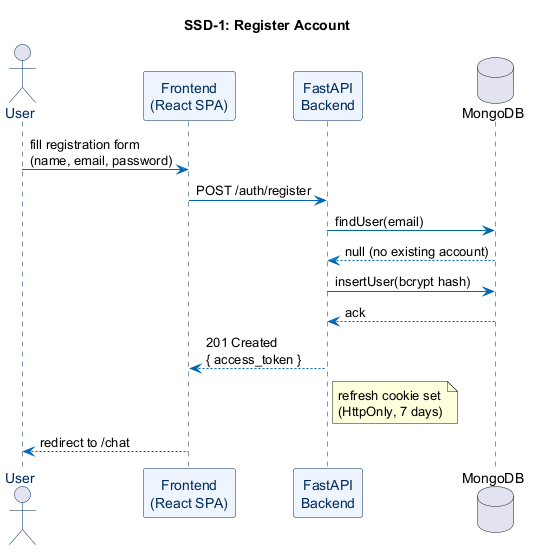
\includegraphics[width=0.85\textwidth]{ssd1_register}
  \caption{SSD-1: Register User Account}
  \label{fig:ssd1}
\end{figure}

%-------------------------------------------------------------
\subsection{SSD-2: Login}
%-------------------------------------------------------------
\begin{figure}[H]
  \centering
  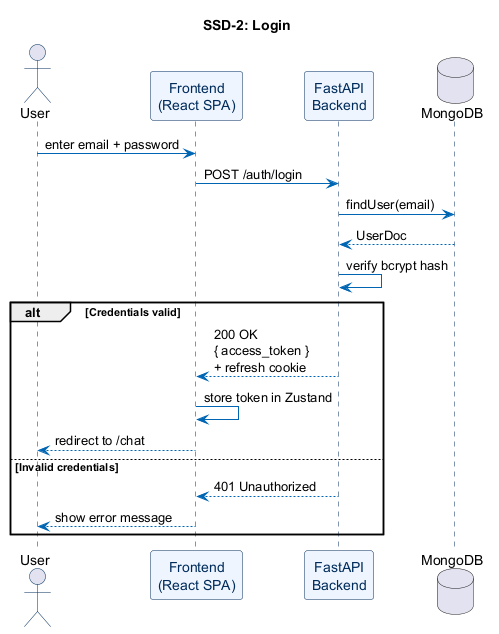
\includegraphics[width=0.85\textwidth]{ssd2_login}
  \caption{SSD-2: Login}
  \label{fig:ssd2}
\end{figure}

%-------------------------------------------------------------
\subsection{SSD-3: Submit Medical Query}
%-------------------------------------------------------------
\begin{figure}[H]
  \centering
  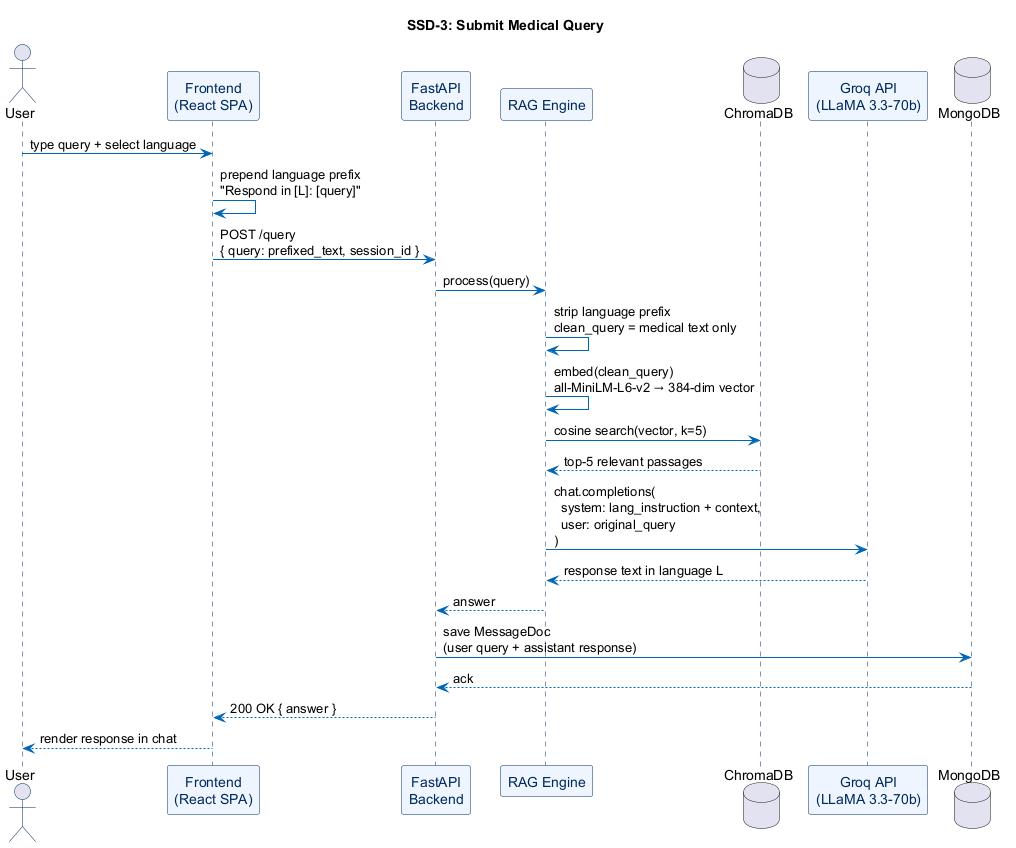
\includegraphics[width=\textwidth]{ssd3_submit_query}
  \caption{SSD-3: Submit Medical Query}
  \label{fig:ssd3}
\end{figure}

%-------------------------------------------------------------
\subsection{SSD-4: Manage Chat Sessions}
%-------------------------------------------------------------
\begin{figure}[H]
  \centering
  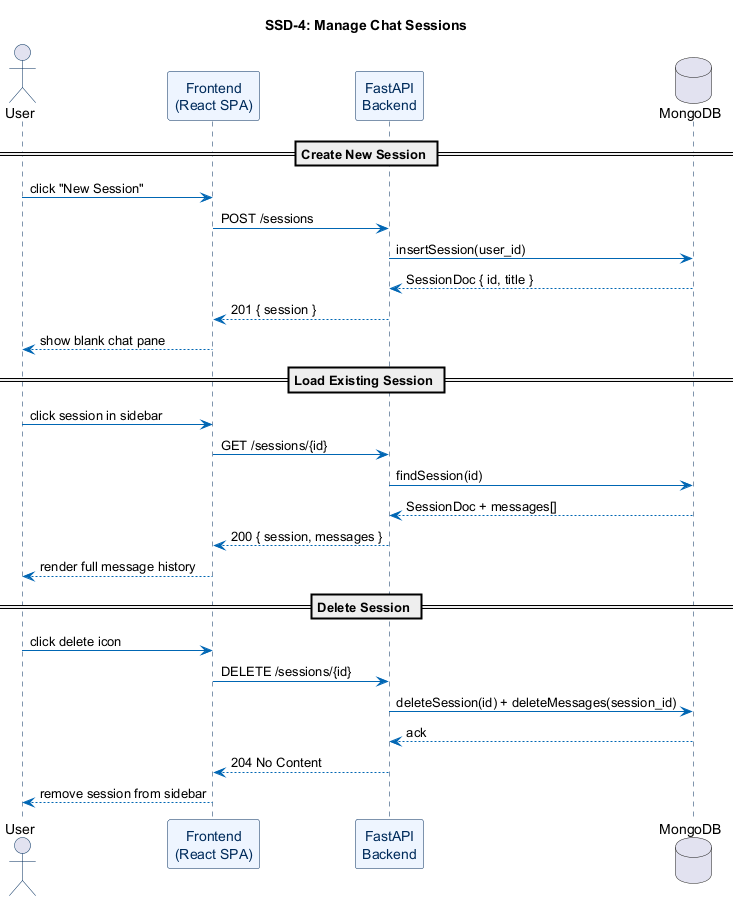
\includegraphics[width=0.90\textwidth]{ssd4_sessions}
  \caption{SSD-4: Manage Chat Sessions (Create / Load / Delete)}
  \label{fig:ssd4}
\end{figure}

%-------------------------------------------------------------
\subsection{SSD-5: Use Voice Input}
%-------------------------------------------------------------
\begin{figure}[H]
  \centering
  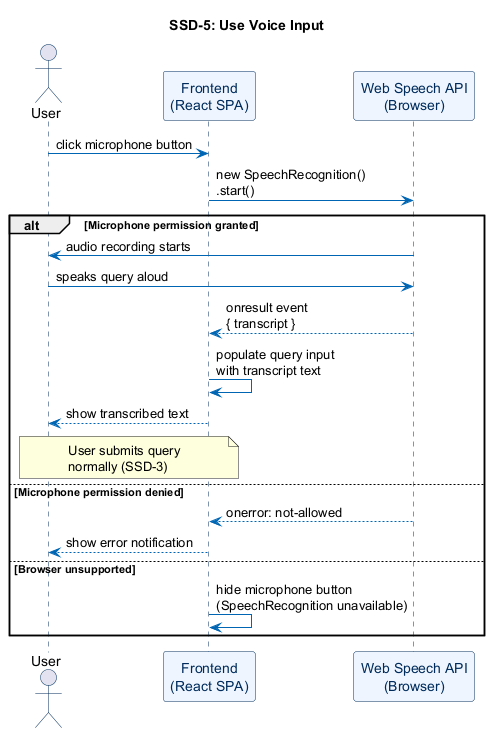
\includegraphics[width=0.85\textwidth]{ssd5_voice_input}
  \caption{SSD-5: Use Voice Input}
  \label{fig:ssd5}
\end{figure}

%-------------------------------------------------------------
\subsection{SSD-6: Use Voice Output}
%-------------------------------------------------------------
\begin{figure}[H]
  \centering
  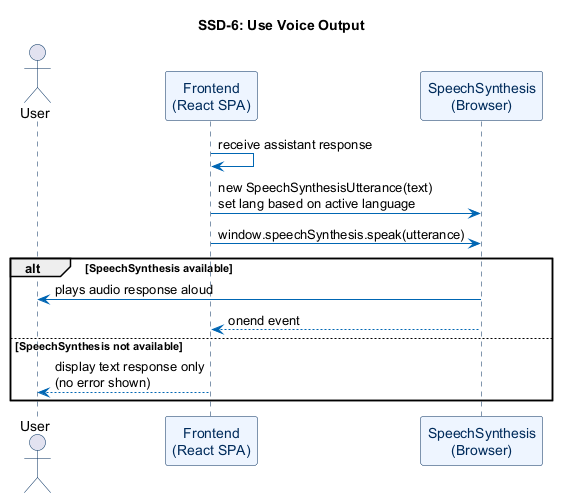
\includegraphics[width=0.75\textwidth]{ssd6_voice_output}
  \caption{SSD-6: Use Voice Output}
  \label{fig:ssd6}
\end{figure}

%-------------------------------------------------------------
\subsection{SSD-7: Manage Profile}
%-------------------------------------------------------------
\begin{figure}[H]
  \centering
  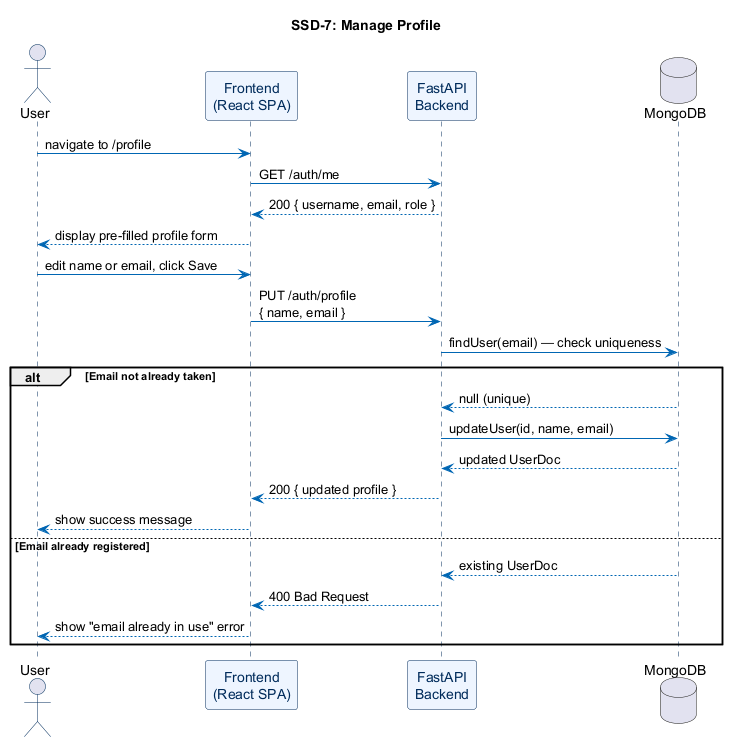
\includegraphics[width=0.85\textwidth]{ssd7_profile}
  \caption{SSD-7: Manage Profile}
  \label{fig:ssd7}
\end{figure}

%-------------------------------------------------------------
\subsection{SSD-8: Reset Password}
%-------------------------------------------------------------
\begin{figure}[H]
  \centering
  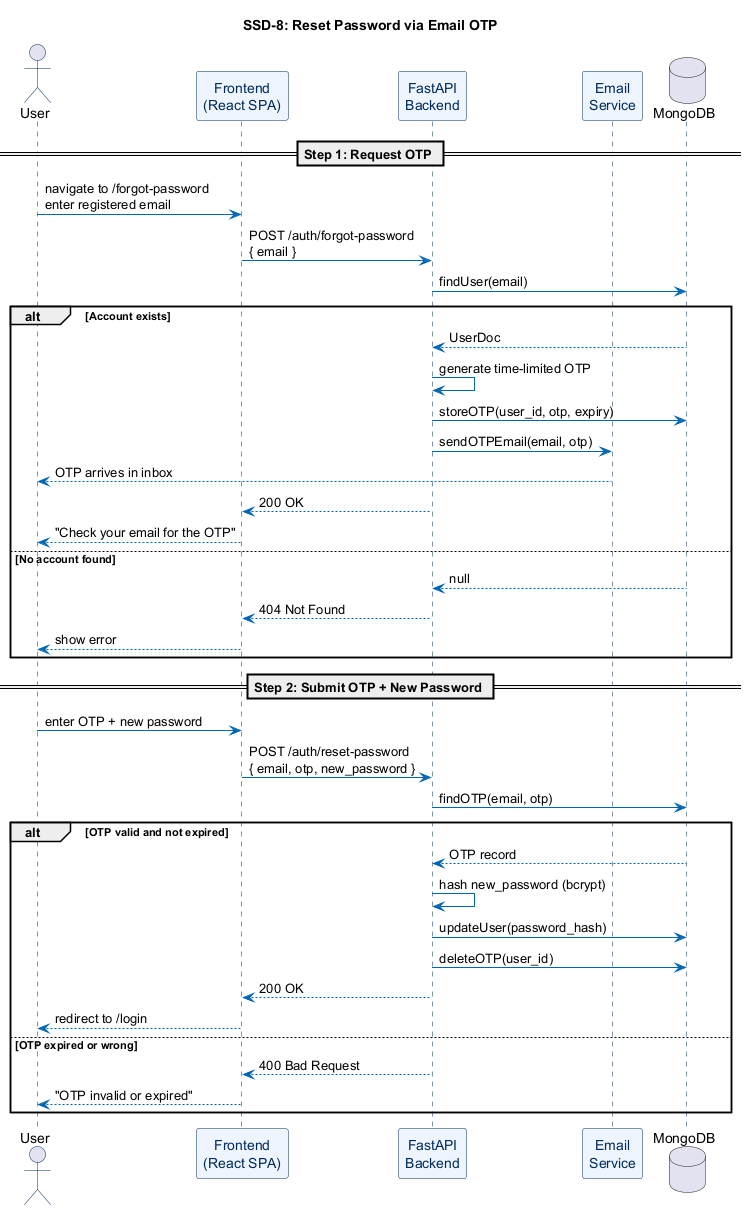
\includegraphics[width=0.90\textwidth]{ssd8_reset_password}
  \caption{SSD-8: Reset Password via Email OTP}
  \label{fig:ssd8}
\end{figure}

%-------------------------------------------------------------
\subsection{SSD-9: Manage Users (Admin)}
%-------------------------------------------------------------
\begin{figure}[H]
  \centering
  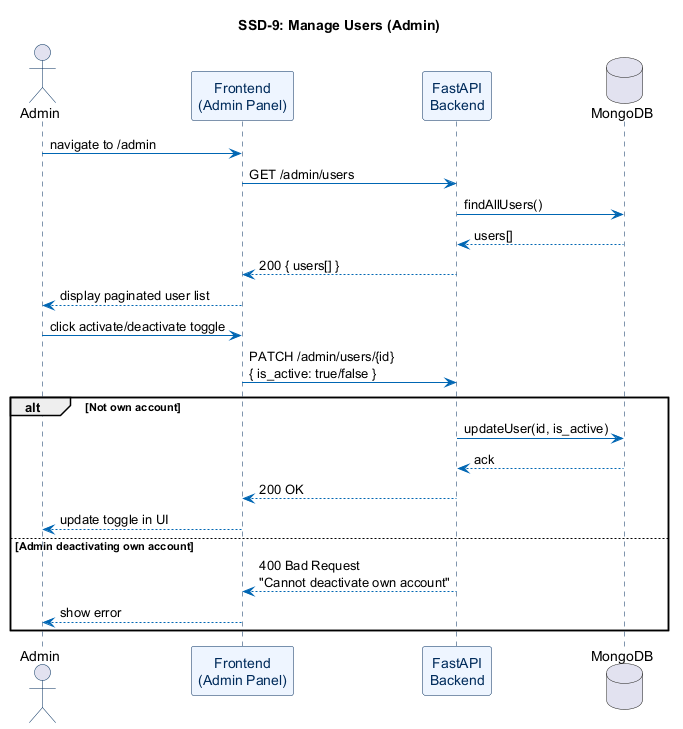
\includegraphics[width=0.85\textwidth]{ssd9_manage_users}
  \caption{SSD-9: Manage Users (Admin)}
  \label{fig:ssd9}
\end{figure}

%-------------------------------------------------------------
\subsection{SSD-10: Ingest Medical Documents (Admin)}
%-------------------------------------------------------------
\begin{figure}[H]
  \centering
  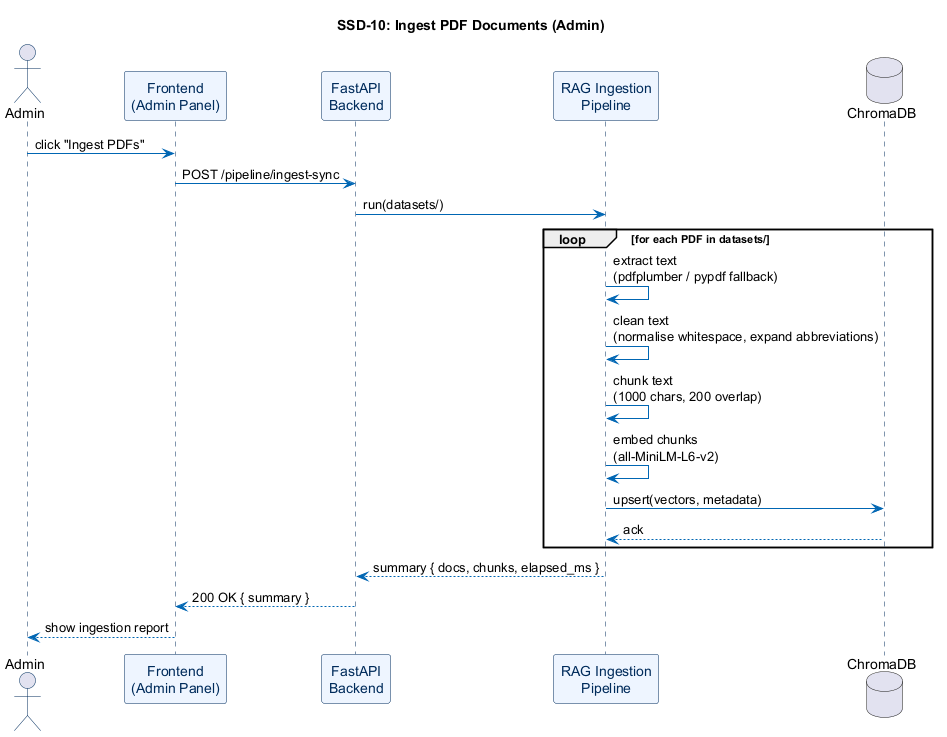
\includegraphics[width=0.90\textwidth]{ssd10_ingest}
  \caption{SSD-10: Ingest Medical Documents (Admin)}
  \label{fig:ssd10}
\end{figure}

%=============================================================
\section{Domain Model}
%=============================================================

The domain model in Figure~\ref{fig:domain} shows the three core persistent entities and
how they relate. The structure is deliberately simple. A \textbf{User} owns zero or more
\textbf{Sessions}. Each \textbf{Session} contains zero or more \textbf{Messages}. When a
session is deleted, everything under it goes with it --- there are no orphaned messages
left behind in the database. All three entities are stored in MongoDB; messages are
embedded inside their parent session document rather than in a separate collection.

\begin{figure}[H]
  \centering
  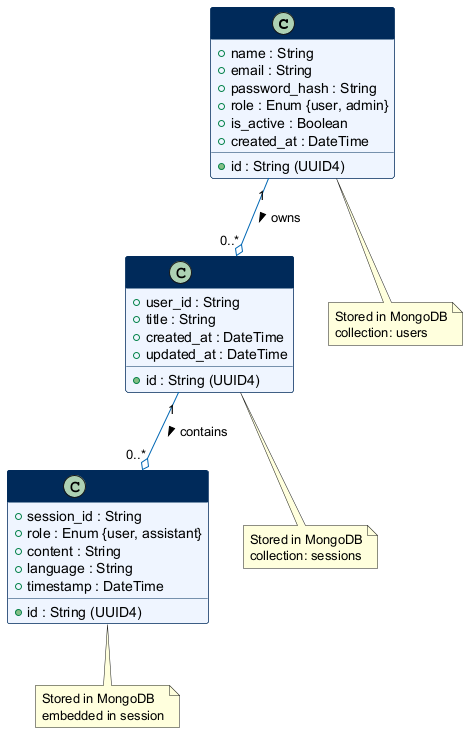
\includegraphics[width=\textwidth]{domain_model}
  \caption{MediLingo AI --- Domain Model}
  \label{fig:domain}
\end{figure}

%============================================================
% CHAPTER 3 -- SOFTWARE DESIGN DESCRIPTION (SDD)
%============================================================

\chapter{Software Design Description (SDD)}

%------------------------------------------------------------
\section{Introduction}
%------------------------------------------------------------

\subsection{Design Overview}

This Software Design Description (SDD) translates the functional and non-functional
requirements from the SRS into concrete structural decisions: how the system is split into
layers and components, how those components interact at runtime, and how persistent data
is organised. The design choices here are not arbitrary --- each one maps back to one or
more requirements, and the traceability matrix in Section~3.1.2 makes those mappings
explicit. The chapter closes with a class diagram covering the key domain entities and
the backend service layer.

MediLingo AI uses a \textbf{three-tier client--server architecture}: a React single-page
application running in the browser, a stateless FastAPI application server, and a dual
persistence layer made up of MongoDB for user and session data and ChromaDB for the indexed
medical knowledge base. The three tiers communicate over HTTPS with JSON payloads; refresh
tokens travel as HTTP-only cookies, keeping them away from JavaScript running in the page.
No business logic lives in the frontend --- the SPA is purely responsible for rendering
state it receives from the API.

\subsection{Requirements Traceability Matrix}

Table~\ref{tab:rtm} maps each functional requirement from the SRS to the design component
responsible for satisfying it, along with the section of this chapter where that component
is described in detail. Any requirement missing a matching row would be a gap in the design.

\begin{longtable}{|>{\bfseries}p{1.8cm}|p{5.2cm}|p{3.8cm}|p{2.0cm}|}
  \caption{Requirements Traceability Matrix}\label{tab:rtm}\\
  \hline
  \theader{Req.\ ID} & \theader{Requirement Summary} & \theader{Design Component} & \theader{Section} \\
  \hline
  \endfirsthead
  \multicolumn{4}{l}{\small\itshape\color{darkgray}(Table \ref{tab:rtm} continued)}\\
  \hline
  \theader{Req.\ ID} & \theader{Requirement Summary} & \theader{Design Component} & \theader{Section} \\
  \hline
  \endhead
  \hline
  \endfoot
  FR-01 & User Registration & Auth Router, UserDoc Model & \ref{sec:auth-router} \\
  \hline
  FR-02 & User Login & Auth Router, JWT Service & \ref{sec:auth-router} \\
  \hline
  FR-03 & Session Persistence (JWT) & Auth Router, apiClient & \ref{sec:auth-router} \\
  \hline
  FR-04 & Logout & Auth Router & \ref{sec:auth-router} \\
  \hline
  FR-05 & Submit Medical Query & Query Router, RAG Engine & \ref{sec:query-router} \\
  \hline
  FR-06 & Language Selection & Frontend Language Store, RAG Engine Prefix Stripping & \ref{sec:frontend} \\
  \hline
  FR-07 & Multilingual Response & RAG Engine, LLM System Prompt & \ref{sec:rag-engine} \\
  \hline
  FR-08 & Retrieve Context Chunks & RAG Engine, Vector Store & \ref{sec:rag-engine} \\
  \hline
  FR-09 & Create Chat Session & Sessions Router, SessionDoc & \ref{sec:sessions-router} \\
  \hline
  FR-10 & Persist Chat History & Sessions Router, MessageDoc & \ref{sec:sessions-router} \\
  \hline
  FR-11 & Load Previous Sessions & Sessions Router & \ref{sec:sessions-router} \\
  \hline
  FR-12 & Delete Session & Sessions Router & \ref{sec:sessions-router} \\
  \hline
  FR-13 & Voice Input & useVoiceInput Hook (Web Speech API) & \ref{sec:frontend} \\
  \hline
  FR-14 & Voice Output & useVoiceOutput Hook (Web Speech API) & \ref{sec:frontend} \\
  \hline
  FR-15 & Admin Login & Auth Router (role check) & \ref{sec:auth-router} \\
  \hline
  FR-16 & PDF Ingestion (Admin) & Pipeline Router, RAG Ingestion Pipeline & \ref{sec:pipeline-router} \\
  \hline
\end{longtable}

%------------------------------------------------------------
\section{System Architectural Design}
%------------------------------------------------------------

\subsection{Chosen System Architecture}

MediLingo AI uses a \textbf{four-tier layered architecture}:

\begin{itemize}
  \item \textbf{Presentation Tier} --- React 19 SPA compiled with Vite, served as static
        files. Talks to the application tier through REST only; no business logic lives here.
        UI state is managed by Zustand stores and voice I/O goes through the browser's
        Web Speech API.

  \item \textbf{Application Tier} --- FastAPI server. Validates requests, enforces
        authentication, coordinates calls to the AI/ML and persistence tiers, and returns
        structured JSON. Stateless by design, which means scaling horizontally is
        straightforward in principle.

  \item \textbf{AI / ML Processing Tier} --- The RAG engine, initialised once at server
        startup and held as a singleton. Handles embedding generation
        (sentence-transformers), vector similarity search (ChromaDB), language-prefix
        stripping, prompt assembly, and LLM invocation (Groq API, LLaMA 3.3-70b). This
        is the most computationally intensive part of the stack.

  \item \textbf{Persistence Tier} --- Two stores: MongoDB (Motor async driver) for user
        accounts, sessions and messages; ChromaDB (local persistence) for the encoded
        medical knowledge base. Both are initialised once at startup via the FastAPI
        lifespan handler.
\end{itemize}

Figure~\ref{fig:arch} presents the system architectural diagram.

% ── System Architectural Diagram ──────────────────────────
\begin{figure}[H]
  \centering
  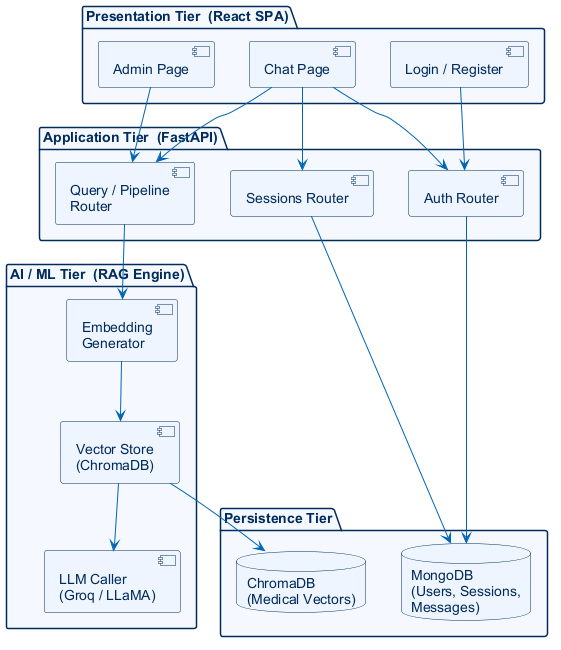
\includegraphics[width=\textwidth]{architecture}
  \caption{MediLingo AI --- Three-Tier System Architecture}
  \label{fig:arch}
\end{figure}

\subsection{Discussion of Alternative Designs}

\subsubsection{Monolithic vs.\ Microservices}

A microservices architecture was evaluated --- separate deployable units for auth, chat,
ingestion and retrieval. It was rejected. The overhead of inter-service communication,
distributed tracing, and individual deployment pipelines is real, and the benefit at this
scale is not. A single developer building an academic prototype does not need Kubernetes.
The layered monolith achieves the same separation of concerns through module boundaries
rather than process boundaries, which is much easier to develop, debug and test.

\subsubsection{Server-Side Rendering vs.\ SPA}

Next.js with server-side rendering was considered as an alternative to the Vite SPA. SSR
improves initial page load and SEO, which matters for public-facing content. MediLingo AI's
chat interface is inherently interactive and session-gated --- there is no content for
search engines to index, no cold visitors landing on a page. The Vite build was preferred:
faster development iteration, simpler deployment as static files, and cleaner integration
with Zustand for keeping access tokens in memory rather than exposing them through
server-rendered HTML.

\subsubsection{Relational vs.\ Document Store}

PostgreSQL with pgvector was a tempting option --- one database handling both relational
user data and vector search. ChromaDB plus MongoDB was chosen instead. ChromaDB's
purpose-built HNSW index and embedding API make the retrieval path significantly
simpler, and MongoDB's flexible schema means the message and session structures can
evolve without writing and running migrations every time something changes. For an
academic project where the schema is still being iterated on, that flexibility mattered.

\subsection{System Interface Description}

\begin{itemize}
  \item \textbf{User Interface} — Browser-based React SPA. Input: text box, microphone
        button, language selector. Output: streamed chat bubbles, text-to-speech playback.

  \item \textbf{API Interface} — REST over HTTP/HTTPS. Base URL
        \texttt{/api/v1}. Authentication via \texttt{Authorization: Bearer <access\_token>}
        header. Refresh via HTTP-only \texttt{refresh\_token} cookie sent automatically
        by the browser.

  \item \textbf{LLM Interface} — Groq REST API. The RAG engine sends a
        \texttt{chat.completions} request containing a system prompt (with language
        instruction and retrieved context) and the user message. Model:
        \texttt{llama-3.3-70b-versatile}.

  \item \textbf{Database Interface} — Motor (async PyMongo) for MongoDB;
        ChromaDB Python client for vector operations. Both connections are initialised
        once at server startup via the FastAPI lifespan handler.
\end{itemize}

%------------------------------------------------------------
\section{Detailed Description of Components}
\label{sec:components}
%------------------------------------------------------------

\subsection{Frontend (React SPA)}
\label{sec:frontend}

The frontend is a React 19 / TypeScript application built with Vite. It is structured
around pages, Zustand stores, and custom hooks that keep side-effectful code away from
the rendering layer. Most components are stateless; they display data received through
props or from the stores, and they call hook functions to trigger any side effects.

\begin{itemize}
  \item \textbf{router.tsx} --- All client-side routes, defined with React Router v6.
        Protected routes check the auth store and redirect to \texttt{/login} when no
        valid access token is present.

  \item \textbf{App.tsx} --- The root component. On mount it silently calls
        \texttt{/auth/refresh}; if the refresh cookie is still valid the access token
        is restored and the user lands directly on the chat page without re-entering
        credentials. This is how the ``stay logged in'' experience works.

  \item \textbf{useAuthStore (Zustand)} --- Holds \texttt{user} and
        \texttt{accessToken} in memory only. Tokens are never written to
        \texttt{localStorage} or \texttt{sessionStorage} --- they disappear when the
        tab closes.

  \item \textbf{apiClient.ts} --- All API calls go through here. It wraps \texttt{fetch}
        with a configurable timeout and handles 401 responses automatically: calls
        \texttt{/auth/refresh}, updates the store, and retries the original request once.
        If the retry also fails, it clears auth state and redirects to \texttt{/login}.

  \item \textbf{useVoiceInput / useVoiceOutput} --- Thin wrappers around
        \texttt{SpeechRecognition} and \texttt{SpeechSynthesis}. The output hook picks
        a locale-appropriate voice based on the active language setting.
\end{itemize}

\subsection{Authentication Router}
\label{sec:auth-router}

\texttt{routers/auth.py} exposes five endpoints under \texttt{/auth}:

\begin{itemize}
  \item \textbf{POST /register} --- Validates uniqueness of both username and email, hashes
        the password with bcrypt via \texttt{passlib}, stores a \texttt{UserDoc} in MongoDB,
        and returns an access/refresh token pair. A duplicate email gets HTTP~400.

  \item \textbf{POST /login} --- Verifies credentials against the stored bcrypt hash and
        issues a new token pair. The refresh token goes into an HTTP-only, Secure,
        SameSite=Lax cookie with a 7-day TTL.

  \item \textbf{POST /refresh} --- Reads the refresh cookie, verifies the JWT signature and
        expiry, then issues a new 15-minute access token. The remaining TTL on the refresh
        token is preserved, not reset.

  \item \textbf{POST /logout} --- Clears the refresh cookie. Nothing else needs to happen
        server-side because access tokens are not persisted anywhere.

  \item \textbf{GET /me} --- Returns the current user's profile using the access token from
        the Authorization header.
\end{itemize}

All tokens are signed HS256 JWTs. The \texttt{SECRET\_KEY} used for signing is loaded
from the environment at startup and is never present in the source code.

\subsection{Sessions Router}
\label{sec:sessions-router}

\texttt{routers/sessions.py} manages chat sessions and their messages under
\texttt{/sessions}. Every endpoint here requires a valid access token.

\begin{itemize}
  \item \textbf{POST /sessions} --- Creates a new \texttt{SessionDoc} in MongoDB with a
        UUID, the authenticated user's ID, a display title and an empty message list.

  \item \textbf{GET /sessions} --- Returns the user's sessions, sorted by last-updated
        descending. This is what populates the sidebar.

  \item \textbf{GET /sessions/\{id\}} --- Returns a single session with its full message
        history. Called when a user clicks on a session to resume it.

  \item \textbf{POST /sessions/\{id\}/messages} --- Appends a \texttt{MessageDoc} (role,
        content, timestamp, language) to the session. Called by the query router after
        each exchange, not directly by the user.

  \item \textbf{DELETE /sessions/\{id\}} --- Deletes the session and all its embedded
        messages.
\end{itemize}

\subsection{Query and Pipeline Routers}
\label{sec:query-router}
\label{sec:pipeline-router}

\texttt{routers/query.py} handles all AI-related endpoints:

\begin{itemize}
  \item \textbf{POST /query} — The primary chat endpoint. Accepts \texttt{query} (the
        full language-prefixed string), strips the prefix, embeds the clean query,
        retrieves the top-\textit{k} context chunks from ChromaDB, assembles the Groq
        prompt, and streams the LLM response back to the caller.

  \item \textbf{POST /retrieve} — Returns only the raw retrieved context chunks, without
        LLM generation. Used for debugging and evaluation.

  \item \textbf{GET /config} — Returns current RAG configuration (chunk size, overlap,
        top-k, model name).

  \item \textbf{GET /info/\{collection\}} — Returns metadata about a ChromaDB collection
        (document count, embedding dimension).
\end{itemize}

\texttt{routers/query.py} also contains pipeline management endpoints under
\texttt{/pipeline}:

\begin{itemize}
  \item \textbf{POST /pipeline/ingest-sync} — Synchronously ingests all PDF files
        found in \texttt{backend/datasets/}. Admin-only. Returns a summary of documents
        indexed, chunks created, and time elapsed.

  \item \textbf{POST /pipeline/ingest} — Same as above but runs as a FastAPI
        \texttt{BackgroundTask}, returning immediately with a task-accepted response.
\end{itemize}

\subsection{RAG Engine}
\label{sec:rag-engine}

The RAG engine (\texttt{rag/engine.py}) is the core AI component of the system.
It is initialised once at server startup through \texttt{services/rag\_service.py} and
held as a module-level singleton. The processing pipeline for each incoming query has
five steps:

\begin{enumerate}
  \item \textbf{Prefix Stripping} --- The language instruction prefix (e.g.,
        \textit{``Respond in Urdu: ''}) is detected and stripped before anything else
        happens. This step is critical for retrieval quality: the clean medical question
        is what gets embedded and searched, not the prefixed string.

  \item \textbf{Embedding} --- The clean query is passed to
        \texttt{EmbeddingGenerator.encode()}, which runs \texttt{all-MiniLM-L6-v2} via
        \texttt{sentence-transformers} to produce a 384-dimensional dense vector.

  \item \textbf{Vector Retrieval} --- The 384-dim query vector is submitted to
        \texttt{ChromaDBVectorStore.query()}, which returns the top-$k$ document chunks
        by cosine similarity.

  \item \textbf{Prompt Assembly} --- A structured Groq chat-completions prompt is built:
        the system message contains the language instruction, a medical-domain persona
        and the retrieved context passages; the user message contains the original
        prefixed query.

  \item \textbf{LLM Invocation} --- The assembled prompt is sent to the Groq API
        (\texttt{llama-3.3-70b-versatile}). The response text is returned to the calling
        router, which saves it to MongoDB and returns it to the frontend.
\end{enumerate}

\subsection{Ingestion Pipeline}
\label{sec:ingestion}

\texttt{rag/pipeline.py} contains \texttt{RAGIngestionPipeline}, which handles the
one-time (or on-demand) process of building the medical knowledge base:

\begin{enumerate}
  \item \textbf{PDF Loading} --- \texttt{rag/loader.py} uses \texttt{pdfplumber} as the
        primary extractor, falling back to \texttt{pypdf} for files that pdfplumber
        cannot handle cleanly. Every PDF in \texttt{backend/datasets/} is processed.

  \item \textbf{Text Cleaning} --- \texttt{rag/preprocessor.py} normalises whitespace,
        expands common medical abbreviations, strips headers and footers, and removes
        non-printable characters. The goal is clean, consistent text going into the
        embedder.

  \item \textbf{Semantic Chunking} --- \texttt{rag/chunker.py} splits cleaned text into
        fixed-size chunks of 1000 characters with 200-character overlap. The overlap
        ensures sentences split across a chunk boundary still appear complete in at
        least one chunk. Short chunks below a minimum length are discarded.

  \item \textbf{Embedding and Indexing} --- Each chunk is embedded and upserted into
        the ChromaDB collection with source filename and chunk index as metadata.
        Upsert rather than insert means re-running the pipeline on an already-indexed
        document does not create duplicates.
\end{enumerate}

\subsection{Data Models}
\label{sec:models}

Three MongoDB document classes are defined in \texttt{models/}:

\begin{itemize}
  \item \textbf{UserDoc} --- \texttt{id} (UUID4 str), \texttt{username}, \texttt{email},
        \texttt{hashed\_password}, \texttt{role} (\textit{user} or \textit{admin}),
        \texttt{created\_at}. Unique indexes on \texttt{username} and \texttt{email} are
        created at startup to enforce deduplication at the database level.

  \item \textbf{SessionDoc} --- \texttt{id} (UUID4 str), \texttt{user\_id},
        \texttt{title}, \texttt{created\_at}, \texttt{updated\_at}, and
        \texttt{messages} --- an embedded array of \texttt{MessageDoc}. The index on
        \texttt{user\_id} makes the ``fetch my sessions'' query fast regardless of
        collection size.

  \item \textbf{MessageDoc} --- \texttt{id} (UUID4 str), \texttt{role} (\textit{user}
        or \textit{assistant}), \texttt{content}, \texttt{language}, \texttt{timestamp}.
        Stored embedded inside \texttt{SessionDoc} rather than in a separate collection.
\end{itemize}

All three models expose \texttt{to\_mongo()} and \texttt{from\_mongo()} helpers.
UUID4 string IDs are used throughout to decouple application identity from MongoDB's
internal \texttt{\_id} field --- application code never touches \texttt{\_id} directly.

%------------------------------------------------------------
\section{Architectural Diagram}
%------------------------------------------------------------

Figure~\ref{fig:arch} in Section~3.2.1 shows the four-tier layered architecture.
Figure~\ref{fig:rag-flow} below zooms in on the AI/ML tier and traces the full
query processing flow from the moment a prefixed query arrives at the RAG engine to
the moment a response is returned to the router.

\begin{figure}[H]
  \centering
  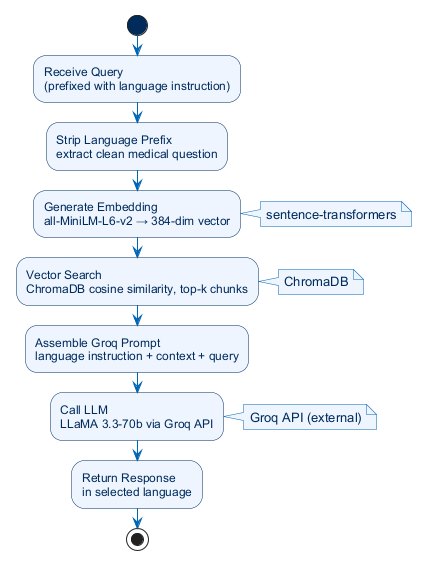
\includegraphics[width=0.55\textwidth]{rag_flow}
  \caption{RAG Query Processing Flow}
  \label{fig:rag-flow}
\end{figure}

%------------------------------------------------------------
\section{Sequence Diagrams}
\label{sec:sequence-diagrams}
%------------------------------------------------------------

This section presents sequence diagrams for each of the ten use cases identified in the
SRS. All ten diagrams are included as exported PNG sequence diagrams.

\subsection{SSD-1: Register Account}

\begin{figure}[H]
  \centering
  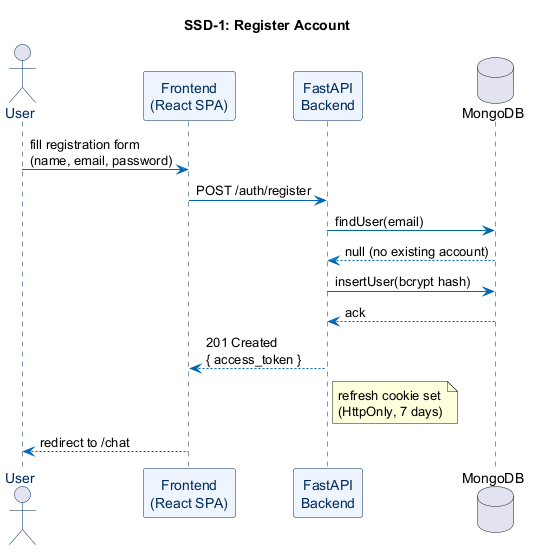
\includegraphics[width=0.85\textwidth]{ssd1_register}
  \caption{SSD-1: Register Account}
  \label{fig:ch3-ssd1}
\end{figure}

\subsection{SSD-2: Login}

\begin{figure}[H]
  \centering
  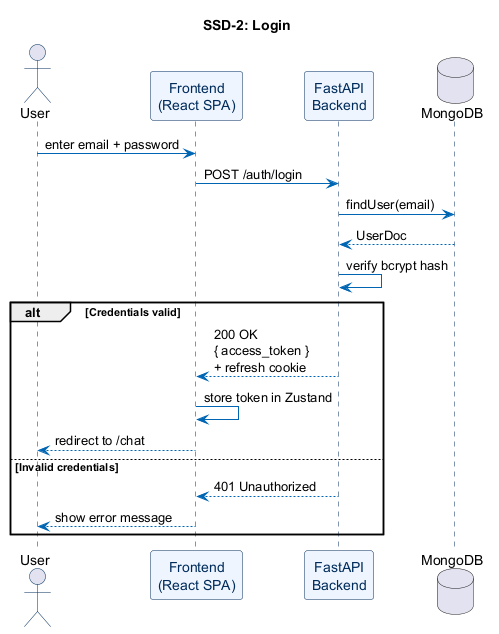
\includegraphics[width=0.85\textwidth]{ssd2_login}
  \caption{SSD-2: Login}
  \label{fig:ch3-ssd2}
\end{figure}

\subsection{SSD-3: Submit Medical Query}

\begin{figure}[H]
  \centering
  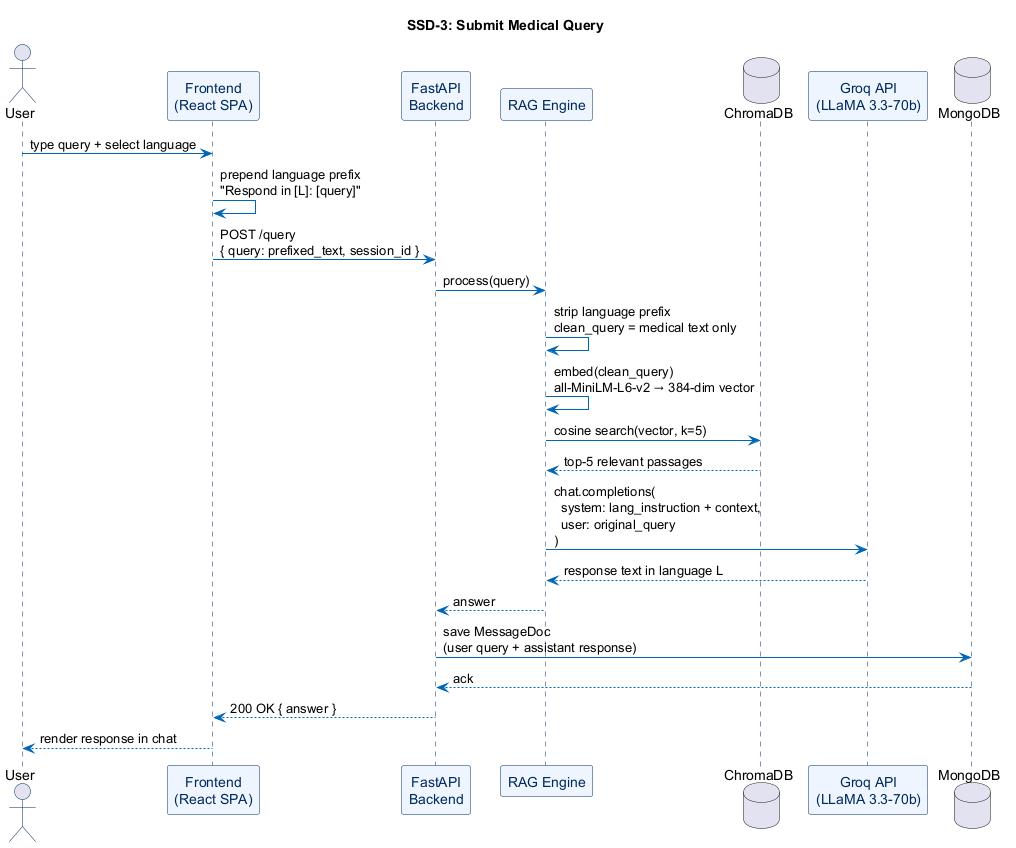
\includegraphics[width=\textwidth]{ssd3_submit_query}
  \caption{SSD-3: Submit Medical Query}
  \label{fig:ch3-ssd3}
\end{figure}

\subsection{SSD-4: Voice Input}

\begin{figure}[H]
  \centering
  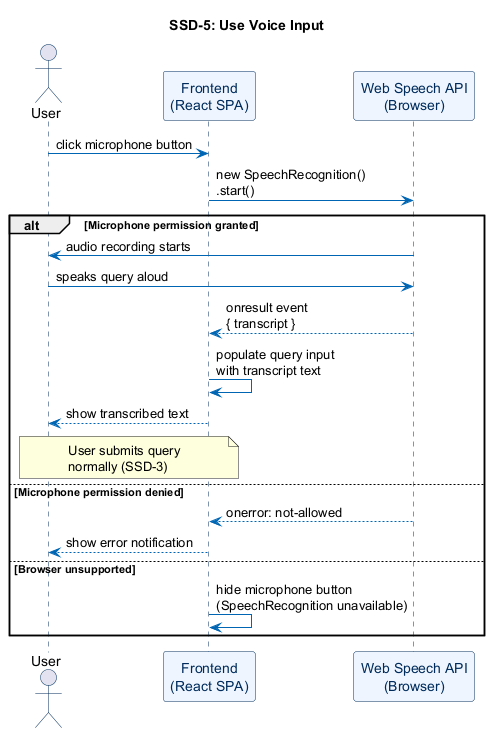
\includegraphics[width=0.85\textwidth]{ssd5_voice_input}
  \caption{SSD-4: Voice Input --- Speech Recognition Flow}
  \label{fig:ch3-ssd4}
\end{figure}

\subsection{SSD-5: Voice Output}

\begin{figure}[H]
  \centering
  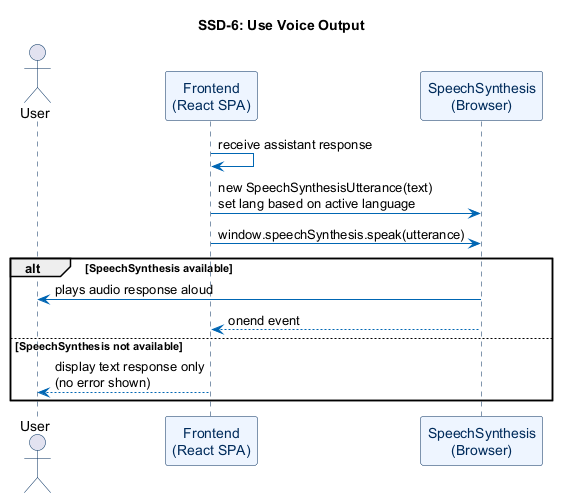
\includegraphics[width=0.85\textwidth]{ssd6_voice_output}
  \caption{SSD-5: Voice Output --- Text-to-Speech Playback Flow}
  \label{fig:ch3-ssd5}
\end{figure}

\subsection{SSD-6: Create New Session}

\begin{figure}[H]
  \centering
  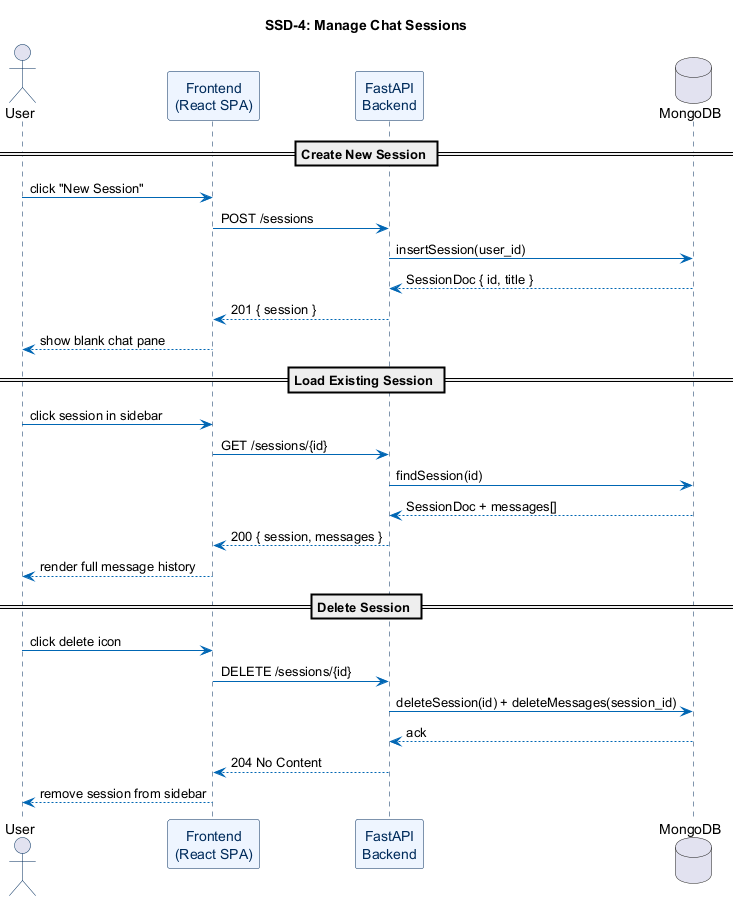
\includegraphics[width=0.85\textwidth]{ssd4_sessions}
  \caption{SSD-6: Create New Session}
  \label{fig:ch3-ssd6}
\end{figure}

\subsection{SSD-7: Load Previous Sessions}

\begin{figure}[H]
  \centering
  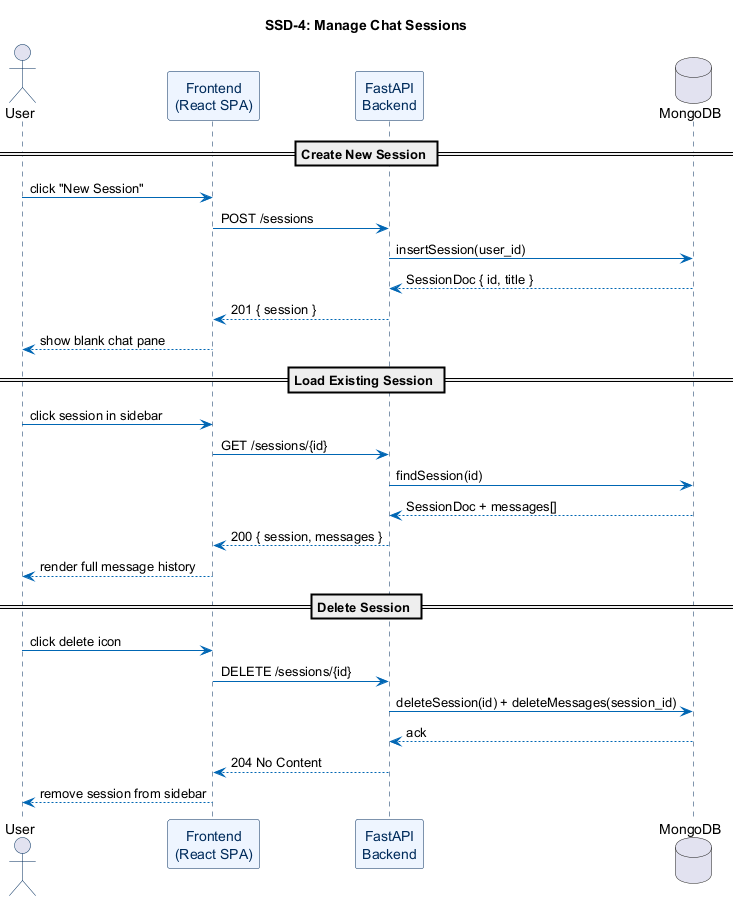
\includegraphics[width=0.90\textwidth]{ssd4_sessions}
  \caption{SSD-7 \& SSD-8: Session Management --- Create, Load, and Delete}
  \label{fig:ch3-ssd7}
\end{figure}

\subsection{SSD-8: Delete Session}

The delete session flow is covered in Figure~\ref{fig:ch3-ssd7} above, which shows all
three session management operations (create, load, and delete) in a single combined
sequence diagram.

\subsection{SSD-9: Admin Login}

\begin{figure}[H]
  \centering
  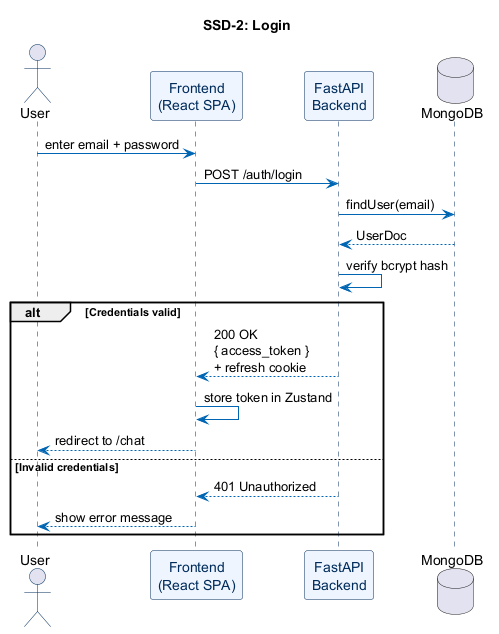
\includegraphics[width=0.85\textwidth]{ssd2_login}
  \caption{SSD-9: Admin Login --- same auth flow as SSD-2, role claim verified server-side}
  \label{fig:ch3-ssd9}
\end{figure}

\subsection{SSD-10: Ingest PDF Documents}

\begin{figure}[H]
  \centering
  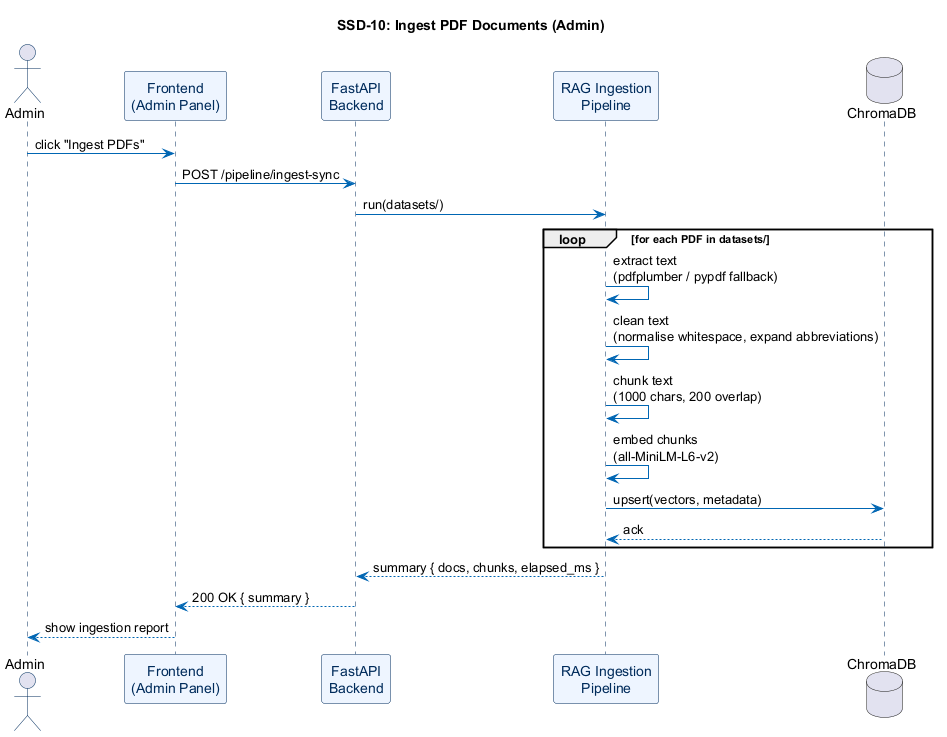
\includegraphics[width=0.90\textwidth]{ssd10_ingest}
  \caption{SSD-10: Ingest PDF Documents}
  \label{fig:ch3-ssd10}
\end{figure}

%------------------------------------------------------------
\section{Class Diagram}
%------------------------------------------------------------

Figure~\ref{fig:class} shows the key domain classes, their attributes and their
relationships. Frontend Zustand stores are left out --- this diagram focuses on the
backend data model and the service layer that drives it. The full picture would include
the React hooks and stores, but adding them here would make the diagram unreadable
without adding much that is not already covered in the frontend component description.

\begin{figure}[H]
  \centering
  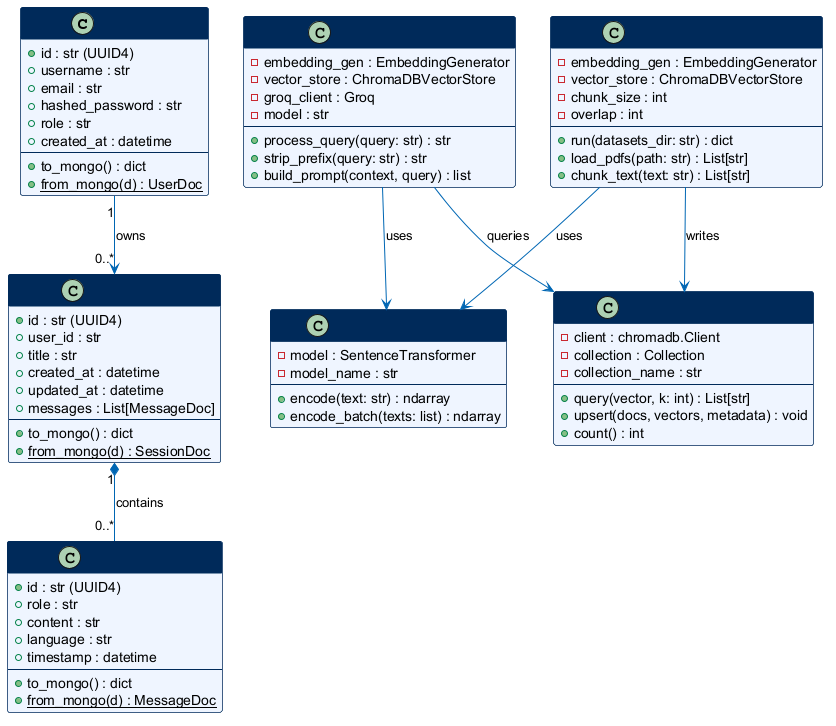
\includegraphics[width=\textwidth]{class_diagram}
  \caption{MediLingo AI --- Class Diagram}
  \label{fig:class}
\end{figure}

%============================================================
% CHAPTER 4 -- SOFTWARE TEST DOCUMENTATION (STD)
%============================================================

\chapter{Software Test Documentation (STD)}

%------------------------------------------------------------
\section{Introduction}
%------------------------------------------------------------

\subsection{System Overview}

Testing any software system is, at its core, about building confidence. Not certainty ---
no test suite can guarantee that --- but enough confidence that the system behaves the way
it was designed to behave under the conditions it will actually face. For MediLingo AI,
that means verifying that a user can register, log in, ask a medical question in Urdu or
English, get a sensible answer back, and have that conversation saved for later. It also
means making sure the admin can upload new PDF documents and that the knowledge base
updates correctly.

The system under test is a full-stack web application: a React frontend talking to a
FastAPI backend, which in turn calls the Groq API and queries ChromaDB. MongoDB stores
everything that needs to persist. Because there are several moving parts here, testing
was done at multiple levels --- individual API endpoints, the authentication flow end to
end, and basic UI interactions through the browser.

\subsection{Test Approach}

The primary testing method was \textbf{black-box functional testing}. Each test case
was written from the perspective of what a user or admin would actually do, not from
knowledge of the internal implementation. The question being asked in every test is
simple: given this input, does the system produce the right output?

Two categories of scenarios were covered for each feature: the \textit{happy path}
(everything goes as expected) and at least one \textit{negative path} (what happens
when something is wrong --- bad credentials, missing fields, duplicate entries, and so
on). Systems that only work when everything is correct are not production-ready, and
that is as true for an academic project as for anything else.

API endpoints were tested directly using Postman, which made it easy to craft specific
request bodies and inspect raw responses without the frontend getting in the way. UI
flows were verified manually in Google Chrome. The RAG pipeline was tested by submitting
known medical queries and checking that the response was grounded in the indexed
documents rather than being a hallucination.

Worth noting: no automated test framework such as Pytest or Vitest was used for these
tests. The test cases documented here represent manual test runs. The pass/fail results
reflect observed system behaviour during the testing phase.

%------------------------------------------------------------
\section{Test Plan}
%------------------------------------------------------------

\subsection{Features to be Tested}

The following features were included in the test scope:

\begin{itemize}
  \item User registration and login, including duplicate account prevention and wrong
        password handling
  \item JWT refresh flow --- specifically, whether an expired access token is
        transparently renewed using the refresh cookie
  \item Logout and session clearing
  \item Submitting medical queries in English, Urdu, and Roman Urdu
  \item Language prefix stripping --- verifying that the embedding pipeline receives
        the clean query, not the prefixed one
  \item Session creation, retrieval, and deletion
  \item Chat history persistence across page reloads
  \item Voice input (speech to text) and voice output (text to speech)
  \item Admin login with role enforcement
  \item PDF ingestion via the admin panel and subsequent retrieval from ChromaDB
\end{itemize}

\subsection{Features Not to be Tested}

Some things are deliberately out of scope:

\begin{itemize}
  \item \textbf{Groq API internals} --- the LLM is an external service. Testing
        whether LLaMA~3.3-70b produces medically accurate responses is beyond the
        scope of this project; what is tested here is whether the system correctly
        calls the API and returns the response to the user.

  \item \textbf{sentence-transformers model accuracy} --- the embedding model is a
        pre-trained open-source model (\texttt{all-MiniLM-L6-v2}). Its retrieval
        quality on general benchmarks is well documented. What is tested here is
        whether the integration works, not the model itself.

  \item \textbf{Cross-browser compatibility} --- testing was done in Chrome only.
        Firefox and Safari compatibility was not verified.

  \item \textbf{Load and stress testing} --- the system was not tested under high
        concurrent user load. This is a single-developer academic prototype, not a
        production service.

  \item \textbf{MongoDB replication or failover} --- a single local MongoDB instance
        was used throughout. Cluster behaviour is outside scope.
\end{itemize}

\subsection{Testing Tools and Environment}

\begin{table}[H]
\centering
\caption{Testing Environment}
\label{tab:env}
\begin{tabularx}{\textwidth}{|l|X|}
\hline
\theader{Component} & \theader{Details} \\
\hline
Operating System    & Windows 11 Home (64-bit) \\
\hline
Browser             & Google Chrome (latest stable) \\
\hline
API Testing Tool    & Postman \\
\hline
Backend Runtime     & Python 3.13, FastAPI with Uvicorn \\
\hline
Frontend Runtime    & Node.js 20, Vite dev server (port 5173) \\
\hline
Database            & MongoDB 7.x (local instance, port 27017) \\
\hline
Vector Store        & ChromaDB (local persistence, \texttt{backend/vectorstore/}) \\
\hline
LLM API             & Groq Cloud (LLaMA 3.3-70b-versatile) \\
\hline
Test PDF            & Sample medical reference document placed in \texttt{backend/datasets/} \\
\hline
\end{tabularx}
\end{table}

%------------------------------------------------------------
\section{Test Cases}
%------------------------------------------------------------

Each use case from the SRS gets at least one positive test and one negative test below.
Test IDs follow the format TC-\textit{UC}-\textit{N}, where \textit{UC} is the use case
number and \textit{N} distinguishes multiple tests within the same use case. Results
reflect observed system behaviour during the testing phase, not theoretical expectations.

%-------------------------------------------------------------
\subsection{UC-1: Register Account}
%-------------------------------------------------------------

\begin{table}[H]
\centering
\caption{TC-01-1: Successful Registration}
\begin{tabularx}{\textwidth}{|l|X|}
\hline
\theader{Field} & \theader{Details} \\
\hline
Test Case ID    & TC-01-1 \\
\hline
Use Case        & UC-1: Register Account \\
\hline
Objective       & Verify that a new user can create an account with valid details \\
\hline
Preconditions   & Backend running; no existing account with the test email \\
\hline
Test Input      & username: \texttt{testuser01}, email: \texttt{testuser01@mail.com},
                  password: \texttt{Test@1234} \\
\hline
Expected Output & HTTP 201; access token returned in response body; refresh cookie set;
                  user redirected to chat page \\
\hline
Actual Result   & Pass \\
\hline
Status          & \textbf{\color{navyblue}Pass} \\
\hline
\end{tabularx}
\end{table}

\begin{table}[H]
\centering
\caption{TC-01-2: Registration with Duplicate Email}
\begin{tabularx}{\textwidth}{|l|X|}
\hline
\theader{Field} & \theader{Details} \\
\hline
Test Case ID    & TC-01-2 \\
\hline
Use Case        & UC-1: Register Account \\
\hline
Objective       & Verify that registering with an already-used email is rejected \\
\hline
Preconditions   & Account with \texttt{testuser01@mail.com} already exists \\
\hline
Test Input      & Same email as TC-01-1 with a different username \\
\hline
Expected Output & HTTP 400; error message indicating email already in use \\
\hline
Actual Result   & Pass \\
\hline
Status          & \textbf{\color{navyblue}Pass} \\
\hline
\end{tabularx}
\end{table}

%-------------------------------------------------------------
\subsection{UC-2: Login}
%-------------------------------------------------------------

\begin{table}[H]
\centering
\caption{TC-02-1: Successful Login}
\begin{tabularx}{\textwidth}{|l|X|}
\hline
\theader{Field} & \theader{Details} \\
\hline
Test Case ID    & TC-02-1 \\
\hline
Use Case        & UC-2: Login \\
\hline
Objective       & Verify that a registered user can log in with correct credentials \\
\hline
Preconditions   & Account from TC-01-1 exists \\
\hline
Test Input      & username: \texttt{testuser01}, password: \texttt{Test@1234} \\
\hline
Expected Output & HTTP 200; access token in body; HttpOnly refresh cookie set;
                  user lands on chat page \\
\hline
Actual Result   & Pass \\
\hline
Status          & \textbf{\color{navyblue}Pass} \\
\hline
\end{tabularx}
\end{table}

\begin{table}[H]
\centering
\caption{TC-02-2: Login with Wrong Password}
\begin{tabularx}{\textwidth}{|l|X|}
\hline
\theader{Field} & \theader{Details} \\
\hline
Test Case ID    & TC-02-2 \\
\hline
Use Case        & UC-2: Login \\
\hline
Objective       & Verify that an incorrect password is rejected \\
\hline
Preconditions   & Account from TC-01-1 exists \\
\hline
Test Input      & username: \texttt{testuser01}, password: \texttt{wrongpass} \\
\hline
Expected Output & HTTP 401; error message: ``Invalid credentials'' \\
\hline
Actual Result   & Pass \\
\hline
Status          & \textbf{\color{navyblue}Pass} \\
\hline
\end{tabularx}
\end{table}

%-------------------------------------------------------------
\subsection{UC-3: Submit Medical Query}
%-------------------------------------------------------------

\begin{table}[H]
\centering
\caption{TC-03-1: English Query}
\begin{tabularx}{\textwidth}{|l|X|}
\hline
\theader{Field} & \theader{Details} \\
\hline
Test Case ID    & TC-03-1 \\
\hline
Use Case        & UC-3: Submit Medical Query \\
\hline
Objective       & Verify that an English medical query returns a relevant, grounded response \\
\hline
Preconditions   & User logged in; at least one PDF ingested into ChromaDB \\
\hline
Test Input      & Language: English; query: ``What are the symptoms of diabetes?'' \\
\hline
Expected Output & HTTP 200; response text in English describing diabetes symptoms;
                  content references retrieved context \\
\hline
Actual Result   & Pass \\
\hline
Status          & \textbf{\color{navyblue}Pass} \\
\hline
\end{tabularx}
\end{table}

\begin{table}[H]
\centering
\caption{TC-03-2: Urdu Query}
\begin{tabularx}{\textwidth}{|l|X|}
\hline
\theader{Field} & \theader{Details} \\
\hline
Test Case ID    & TC-03-2 \\
\hline
Use Case        & UC-3: Submit Medical Query \\
\hline
Objective       & Verify that an Urdu query returns a response written in Urdu \\
\hline
Preconditions   & User logged in; language selector set to Urdu \\
\hline
Test Input      & Language: Urdu; query: \textit{(What are the symptoms of diabetes? --- written in Urdu script)} \\
\hline
Expected Output & Response text in Urdu script; semantically correct answer \\
\hline
Actual Result   & Pass \\
\hline
Status          & \textbf{\color{navyblue}Pass} \\
\hline
\end{tabularx}
\end{table}

\begin{table}[H]
\centering
\caption{TC-03-3: Roman Urdu Query}
\begin{tabularx}{\textwidth}{|l|X|}
\hline
\theader{Field} & \theader{Details} \\
\hline
Test Case ID    & TC-03-3 \\
\hline
Use Case        & UC-3: Submit Medical Query \\
\hline
Objective       & Verify that a Roman Urdu query returns a response in Roman Urdu \\
\hline
Preconditions   & User logged in; language selector set to Roman Urdu \\
\hline
Test Input      & Language: Roman Urdu; query: ``Diabetes ki alamaat kya hain?'' \\
\hline
Expected Output & Response written in Roman Urdu; content correct \\
\hline
Actual Result   & Pass \\
\hline
Status          & \textbf{\color{navyblue}Pass} \\
\hline
\end{tabularx}
\end{table}

\begin{table}[H]
\centering
\caption{TC-03-4: Query Without Ingested Documents}
\begin{tabularx}{\textwidth}{|l|X|}
\hline
\theader{Field} & \theader{Details} \\
\hline
Test Case ID    & TC-03-4 \\
\hline
Use Case        & UC-3: Submit Medical Query \\
\hline
Objective       & Verify graceful handling when the vector store is empty \\
\hline
Preconditions   & ChromaDB collection empty (no ingestion run yet) \\
\hline
Test Input      & Any valid medical query \\
\hline
Expected Output & System responds with a message indicating no context is available;
                  does not crash \\
\hline
Actual Result   & Pass \\
\hline
Status          & \textbf{\color{navyblue}Pass} \\
\hline
\end{tabularx}
\end{table}

%-------------------------------------------------------------
\subsection{UC-4: Voice Input}
%-------------------------------------------------------------

\begin{table}[H]
\centering
\caption{TC-04-1: Voice Input in English}
\begin{tabularx}{\textwidth}{|l|X|}
\hline
\theader{Field} & \theader{Details} \\
\hline
Test Case ID    & TC-04-1 \\
\hline
Use Case        & UC-4: Voice Input \\
\hline
Objective       & Verify that speech is correctly transcribed and placed in the query box \\
\hline
Preconditions   & Chrome browser; microphone permission granted; language set to English \\
\hline
Test Input      & Spoken: ``What is hypertension?'' \\
\hline
Expected Output & Query box populated with transcribed text; query submittable \\
\hline
Actual Result   & Pass \\
\hline
Status          & \textbf{\color{navyblue}Pass} \\
\hline
\end{tabularx}
\end{table}

\begin{table}[H]
\centering
\caption{TC-04-2: Microphone Permission Denied}
\begin{tabularx}{\textwidth}{|l|X|}
\hline
\theader{Field} & \theader{Details} \\
\hline
Test Case ID    & TC-04-2 \\
\hline
Use Case        & UC-4: Voice Input \\
\hline
Objective       & Verify the app handles microphone permission denial gracefully \\
\hline
Preconditions   & Microphone permission blocked in Chrome settings \\
\hline
Test Input      & Click microphone button \\
\hline
Expected Output & Error notification shown to user; app does not crash \\
\hline
Actual Result   & Pass \\
\hline
Status          & \textbf{\color{navyblue}Pass} \\
\hline
\end{tabularx}
\end{table}

%-------------------------------------------------------------
\subsection{UC-5: Voice Output}
%-------------------------------------------------------------

\begin{table}[H]
\centering
\caption{TC-05-1: Text-to-Speech Playback}
\begin{tabularx}{\textwidth}{|l|X|}
\hline
\theader{Field} & \theader{Details} \\
\hline
Test Case ID    & TC-05-1 \\
\hline
Use Case        & UC-5: Voice Output \\
\hline
Objective       & Verify that the system reads out the assistant response after it arrives \\
\hline
Preconditions   & User logged in; a query has just been submitted and answered \\
\hline
Test Input      & Language: English; response received from the system \\
\hline
Expected Output & Browser TTS reads the response aloud using an English voice \\
\hline
Actual Result   & Pass \\
\hline
Status          & \textbf{\color{navyblue}Pass} \\
\hline
\end{tabularx}
\end{table}

%-------------------------------------------------------------
\subsection{UC-6: Create New Session}
%-------------------------------------------------------------

\begin{table}[H]
\centering
\caption{TC-06-1: Create a New Chat Session}
\begin{tabularx}{\textwidth}{|l|X|}
\hline
\theader{Field} & \theader{Details} \\
\hline
Test Case ID    & TC-06-1 \\
\hline
Use Case        & UC-6: Create New Session \\
\hline
Objective       & Verify that clicking New Session creates a blank session in the sidebar \\
\hline
Preconditions   & User is logged in and on the chat page \\
\hline
Test Input      & Click the ``New Session'' button \\
\hline
Expected Output & New session appears in sidebar; chat area is blank;
                  session ID stored in MongoDB \\
\hline
Actual Result   & Pass \\
\hline
Status          & \textbf{\color{navyblue}Pass} \\
\hline
\end{tabularx}
\end{table}

%-------------------------------------------------------------
\subsection{UC-7: Load Previous Sessions}
%-------------------------------------------------------------

\begin{table}[H]
\centering
\caption{TC-07-1: Reload Previous Session After Page Refresh}
\begin{tabularx}{\textwidth}{|l|X|}
\hline
\theader{Field} & \theader{Details} \\
\hline
Test Case ID    & TC-07-1 \\
\hline
Use Case        & UC-7: Load Previous Sessions \\
\hline
Objective       & Verify that a session with prior messages loads correctly after a full page reload \\
\hline
Preconditions   & User has an existing session with at least two messages \\
\hline
Test Input      & Refresh page; click on the session in the sidebar \\
\hline
Expected Output & Full message history displayed in the correct order; no messages missing \\
\hline
Actual Result   & Pass \\
\hline
Status          & \textbf{\color{navyblue}Pass} \\
\hline
\end{tabularx}
\end{table}

%-------------------------------------------------------------
\subsection{UC-8: Delete Session}
%-------------------------------------------------------------

\begin{table}[H]
\centering
\caption{TC-08-1: Delete an Existing Session}
\begin{tabularx}{\textwidth}{|l|X|}
\hline
\theader{Field} & \theader{Details} \\
\hline
Test Case ID    & TC-08-1 \\
\hline
Use Case        & UC-8: Delete Session \\
\hline
Objective       & Verify that deleting a session removes it from the sidebar and from MongoDB \\
\hline
Preconditions   & User has at least one existing session \\
\hline
Test Input      & Click the delete icon next to a session \\
\hline
Expected Output & Session disappears from sidebar; GET /sessions no longer returns it;
                  MongoDB record deleted \\
\hline
Actual Result   & Pass \\
\hline
Status          & \textbf{\color{navyblue}Pass} \\
\hline
\end{tabularx}
\end{table}

\begin{table}[H]
\centering
\caption{TC-08-2: Delete with Invalid Session ID}
\begin{tabularx}{\textwidth}{|l|X|}
\hline
\theader{Field} & \theader{Details} \\
\hline
Test Case ID    & TC-08-2 \\
\hline
Use Case        & UC-8: Delete Session \\
\hline
Objective       & Verify that a DELETE request with a non-existent session ID is handled gracefully \\
\hline
Preconditions   & User authenticated \\
\hline
Test Input      & DELETE /sessions/\texttt{nonexistent-id-12345} \\
\hline
Expected Output & HTTP 404; error message returned; no crash \\
\hline
Actual Result   & Pass \\
\hline
Status          & \textbf{\color{navyblue}Pass} \\
\hline
\end{tabularx}
\end{table}

%-------------------------------------------------------------
\subsection{UC-9: Admin Login}
%-------------------------------------------------------------

\begin{table}[H]
\centering
\caption{TC-09-1: Admin Login with Valid Credentials}
\begin{tabularx}{\textwidth}{|l|X|}
\hline
\theader{Field} & \theader{Details} \\
\hline
Test Case ID    & TC-09-1 \\
\hline
Use Case        & UC-9: Admin Login \\
\hline
Objective       & Verify that a user with admin role can access the admin dashboard \\
\hline
Preconditions   & Admin account exists in MongoDB with \texttt{role: "admin"} \\
\hline
Test Input      & Admin username and password on the /admin/login page \\
\hline
Expected Output & Login succeeds; admin dashboard rendered; access token contains admin role \\
\hline
Actual Result   & Pass \\
\hline
Status          & \textbf{\color{navyblue}Pass} \\
\hline
\end{tabularx}
\end{table}

\begin{table}[H]
\centering
\caption{TC-09-2: Regular User Cannot Access Admin Routes}
\begin{tabularx}{\textwidth}{|l|X|}
\hline
\theader{Field} & \theader{Details} \\
\hline
Test Case ID    & TC-09-2 \\
\hline
Use Case        & UC-9: Admin Login \\
\hline
Objective       & Verify that a regular user token is rejected on admin-only endpoints \\
\hline
Preconditions   & Logged in as a non-admin user; access token obtained \\
\hline
Test Input      & POST /pipeline/ingest-sync with non-admin token in Authorization header \\
\hline
Expected Output & HTTP 403 Forbidden; access denied message \\
\hline
Actual Result   & Pass \\
\hline
Status          & \textbf{\color{navyblue}Pass} \\
\hline
\end{tabularx}
\end{table}

%-------------------------------------------------------------
\subsection{UC-10: Ingest PDF Documents}
%-------------------------------------------------------------

\begin{table}[H]
\centering
\caption{TC-10-1: Successful PDF Ingestion}
\begin{tabularx}{\textwidth}{|l|X|}
\hline
\theader{Field} & \theader{Details} \\
\hline
Test Case ID    & TC-10-1 \\
\hline
Use Case        & UC-10: Ingest PDF Documents \\
\hline
Objective       & Verify that a valid PDF placed in the datasets folder is indexed into ChromaDB \\
\hline
Preconditions   & Admin logged in; at least one PDF in \texttt{backend/datasets/};
                  ChromaDB running \\
\hline
Test Input      & Click ``Ingest PDFs'' on the admin panel (POST /pipeline/ingest-sync) \\
\hline
Expected Output & HTTP 200; response body shows document count, chunk count, and elapsed
                  time; queries against the indexed content now return relevant results \\
\hline
Actual Result   & Pass \\
\hline
Status          & \textbf{\color{navyblue}Pass} \\
\hline
\end{tabularx}
\end{table}

\begin{table}[H]
\centering
\caption{TC-10-2: Ingestion with Empty Datasets Folder}
\begin{tabularx}{\textwidth}{|l|X|}
\hline
\theader{Field} & \theader{Details} \\
\hline
Test Case ID    & TC-10-2 \\
\hline
Use Case        & UC-10: Ingest PDF Documents \\
\hline
Objective       & Verify that the ingestion endpoint handles an empty folder without crashing \\
\hline
Preconditions   & Admin logged in; \texttt{backend/datasets/} folder is empty \\
\hline
Test Input      & POST /pipeline/ingest-sync \\
\hline
Expected Output & HTTP 200; response body indicates 0 documents processed; no error \\
\hline
Actual Result   & Pass \\
\hline
Status          & \textbf{\color{navyblue}Pass} \\
\hline
\end{tabularx}
\end{table}

%-------------------------------------------------------------
\subsection{Test Summary}
%-------------------------------------------------------------

Table~\ref{tab:summary} gives a consolidated view of every test case run and the result.

\begin{longtable}{|l|l|p{5.2cm}|l|}
  \caption{Test Execution Summary}\label{tab:summary}\\
  \hline
  \theader{TC ID} & \theader{Use Case} & \theader{Objective (brief)} & \theader{Status} \\
  \hline
  \endfirsthead
  \multicolumn{4}{l}{\small\itshape\color{darkgray}(Table \ref{tab:summary} continued)}\\
  \hline
  \theader{TC ID} & \theader{Use Case} & \theader{Objective (brief)} & \theader{Status} \\
  \hline
  \endhead
  \hline
  \endfoot
  TC-01-1 & Register Account  & Valid registration succeeds             & \textbf{Pass} \\ \hline
  TC-01-2 & Register Account  & Duplicate email rejected                & \textbf{Pass} \\ \hline
  TC-02-1 & Login             & Correct credentials accepted            & \textbf{Pass} \\ \hline
  TC-02-2 & Login             & Wrong password rejected                 & \textbf{Pass} \\ \hline
  TC-03-1 & Submit Query      & English query returns English answer    & \textbf{Pass} \\ \hline
  TC-03-2 & Submit Query      & Urdu query returns Urdu answer          & \textbf{Pass} \\ \hline
  TC-03-3 & Submit Query      & Roman Urdu query handled correctly      & \textbf{Pass} \\ \hline
  TC-03-4 & Submit Query      & Empty vector store handled gracefully   & \textbf{Pass} \\ \hline
  TC-04-1 & Voice Input       & Speech transcribed to query box         & \textbf{Pass} \\ \hline
  TC-04-2 & Voice Input       & Mic denial handled without crash        & \textbf{Pass} \\ \hline
  TC-05-1 & Voice Output      & Response read aloud via TTS             & \textbf{Pass} \\ \hline
  TC-06-1 & Create Session    & New session created and shown           & \textbf{Pass} \\ \hline
  TC-07-1 & Load Sessions     & History reloads correctly after refresh & \textbf{Pass} \\ \hline
  TC-08-1 & Delete Session    & Session removed from DB and UI          & \textbf{Pass} \\ \hline
  TC-08-2 & Delete Session    & Invalid ID returns 404                  & \textbf{Pass} \\ \hline
  TC-09-1 & Admin Login       & Admin accesses dashboard                & \textbf{Pass} \\ \hline
  TC-09-2 & Admin Login       & Regular user blocked from admin routes  & \textbf{Pass} \\ \hline
  TC-10-1 & PDF Ingestion     & PDF indexed into ChromaDB               & \textbf{Pass} \\ \hline
  TC-10-2 & PDF Ingestion     & Empty folder returns zero docs, no crash & \textbf{Pass} \\ \hline
\end{longtable}

All 19 test cases passed. The core RAG flow --- query in, response out, same language ---
worked correctly in all three languages. The JWT lifecycle behaved as designed: expired
access tokens were transparently renewed from the refresh cookie without the user
noticing. Role enforcement held up: a non-admin token was correctly rejected on the
admin ingestion endpoint. The ingestion pipeline handled both the happy path and the
empty-folder edge case without errors. There were no unexpected crashes or unhandled
exceptions observed during any of the test runs.


%-------------------------------------------------------------
% REFERENCES
%-------------------------------------------------------------
\clearpage
\addcontentsline{toc}{chapter}{REFERENCES}
\bibliographystyle{ieeetr}
\bibliography{references}

\end{document}
